% Options for packages loaded elsewhere
\PassOptionsToPackage{unicode}{hyperref}
\PassOptionsToPackage{hyphens}{url}
%
\documentclass[
]{article}
\usepackage{amsmath,amssymb}
\usepackage{lmodern}
\usepackage{iftex}
\ifPDFTeX
  \usepackage[T1]{fontenc}
  \usepackage[utf8]{inputenc}
  \usepackage{textcomp} % provide euro and other symbols
\else % if luatex or xetex
  \usepackage{unicode-math}
  \defaultfontfeatures{Scale=MatchLowercase}
  \defaultfontfeatures[\rmfamily]{Ligatures=TeX,Scale=1}
\fi
% Use upquote if available, for straight quotes in verbatim environments
\IfFileExists{upquote.sty}{\usepackage{upquote}}{}
\IfFileExists{microtype.sty}{% use microtype if available
  \usepackage[]{microtype}
  \UseMicrotypeSet[protrusion]{basicmath} % disable protrusion for tt fonts
}{}
\makeatletter
\@ifundefined{KOMAClassName}{% if non-KOMA class
  \IfFileExists{parskip.sty}{%
    \usepackage{parskip}
  }{% else
    \setlength{\parindent}{0pt}
    \setlength{\parskip}{6pt plus 2pt minus 1pt}}
}{% if KOMA class
  \KOMAoptions{parskip=half}}
\makeatother
\usepackage{xcolor}
\usepackage[margin=1in]{geometry}
\usepackage{color}
\usepackage{fancyvrb}
\newcommand{\VerbBar}{|}
\newcommand{\VERB}{\Verb[commandchars=\\\{\}]}
\DefineVerbatimEnvironment{Highlighting}{Verbatim}{commandchars=\\\{\}}
% Add ',fontsize=\small' for more characters per line
\usepackage{framed}
\definecolor{shadecolor}{RGB}{248,248,248}
\newenvironment{Shaded}{\begin{snugshade}}{\end{snugshade}}
\newcommand{\AlertTok}[1]{\textcolor[rgb]{0.94,0.16,0.16}{#1}}
\newcommand{\AnnotationTok}[1]{\textcolor[rgb]{0.56,0.35,0.01}{\textbf{\textit{#1}}}}
\newcommand{\AttributeTok}[1]{\textcolor[rgb]{0.77,0.63,0.00}{#1}}
\newcommand{\BaseNTok}[1]{\textcolor[rgb]{0.00,0.00,0.81}{#1}}
\newcommand{\BuiltInTok}[1]{#1}
\newcommand{\CharTok}[1]{\textcolor[rgb]{0.31,0.60,0.02}{#1}}
\newcommand{\CommentTok}[1]{\textcolor[rgb]{0.56,0.35,0.01}{\textit{#1}}}
\newcommand{\CommentVarTok}[1]{\textcolor[rgb]{0.56,0.35,0.01}{\textbf{\textit{#1}}}}
\newcommand{\ConstantTok}[1]{\textcolor[rgb]{0.00,0.00,0.00}{#1}}
\newcommand{\ControlFlowTok}[1]{\textcolor[rgb]{0.13,0.29,0.53}{\textbf{#1}}}
\newcommand{\DataTypeTok}[1]{\textcolor[rgb]{0.13,0.29,0.53}{#1}}
\newcommand{\DecValTok}[1]{\textcolor[rgb]{0.00,0.00,0.81}{#1}}
\newcommand{\DocumentationTok}[1]{\textcolor[rgb]{0.56,0.35,0.01}{\textbf{\textit{#1}}}}
\newcommand{\ErrorTok}[1]{\textcolor[rgb]{0.64,0.00,0.00}{\textbf{#1}}}
\newcommand{\ExtensionTok}[1]{#1}
\newcommand{\FloatTok}[1]{\textcolor[rgb]{0.00,0.00,0.81}{#1}}
\newcommand{\FunctionTok}[1]{\textcolor[rgb]{0.00,0.00,0.00}{#1}}
\newcommand{\ImportTok}[1]{#1}
\newcommand{\InformationTok}[1]{\textcolor[rgb]{0.56,0.35,0.01}{\textbf{\textit{#1}}}}
\newcommand{\KeywordTok}[1]{\textcolor[rgb]{0.13,0.29,0.53}{\textbf{#1}}}
\newcommand{\NormalTok}[1]{#1}
\newcommand{\OperatorTok}[1]{\textcolor[rgb]{0.81,0.36,0.00}{\textbf{#1}}}
\newcommand{\OtherTok}[1]{\textcolor[rgb]{0.56,0.35,0.01}{#1}}
\newcommand{\PreprocessorTok}[1]{\textcolor[rgb]{0.56,0.35,0.01}{\textit{#1}}}
\newcommand{\RegionMarkerTok}[1]{#1}
\newcommand{\SpecialCharTok}[1]{\textcolor[rgb]{0.00,0.00,0.00}{#1}}
\newcommand{\SpecialStringTok}[1]{\textcolor[rgb]{0.31,0.60,0.02}{#1}}
\newcommand{\StringTok}[1]{\textcolor[rgb]{0.31,0.60,0.02}{#1}}
\newcommand{\VariableTok}[1]{\textcolor[rgb]{0.00,0.00,0.00}{#1}}
\newcommand{\VerbatimStringTok}[1]{\textcolor[rgb]{0.31,0.60,0.02}{#1}}
\newcommand{\WarningTok}[1]{\textcolor[rgb]{0.56,0.35,0.01}{\textbf{\textit{#1}}}}
\usepackage{graphicx}
\makeatletter
\def\maxwidth{\ifdim\Gin@nat@width>\linewidth\linewidth\else\Gin@nat@width\fi}
\def\maxheight{\ifdim\Gin@nat@height>\textheight\textheight\else\Gin@nat@height\fi}
\makeatother
% Scale images if necessary, so that they will not overflow the page
% margins by default, and it is still possible to overwrite the defaults
% using explicit options in \includegraphics[width, height, ...]{}
\setkeys{Gin}{width=\maxwidth,height=\maxheight,keepaspectratio}
% Set default figure placement to htbp
\makeatletter
\def\fps@figure{htbp}
\makeatother
\setlength{\emergencystretch}{3em} % prevent overfull lines
\providecommand{\tightlist}{%
  \setlength{\itemsep}{0pt}\setlength{\parskip}{0pt}}
\setcounter{secnumdepth}{-\maxdimen} % remove section numbering
\ifLuaTeX
  \usepackage{selnolig}  % disable illegal ligatures
\fi
\IfFileExists{bookmark.sty}{\usepackage{bookmark}}{\usepackage{hyperref}}
\IfFileExists{xurl.sty}{\usepackage{xurl}}{} % add URL line breaks if available
\urlstyle{same} % disable monospaced font for URLs
\hypersetup{
  pdftitle={Sampling distributions/uncertainty},
  pdfauthor={NRES 710},
  hidelinks,
  pdfcreator={LaTeX via pandoc}}

\title{Sampling distributions/uncertainty}
\author{NRES 710}
\date{Fall 2022}

\begin{document}
\maketitle

\hypertarget{download-the-r-code-for-this-lecture}{%
\subsection{Download the R code for this
lecture!}\label{download-the-r-code-for-this-lecture}}

To follow along with the R-based lessons and demos,
\href{LECTURE2.R}{right (or command) click on this link and save the
script to your working directory}

\hypertarget{statistics-inference-from-a-sample}{%
\subsection{Statistics: inference from a
sample}\label{statistics-inference-from-a-sample}}

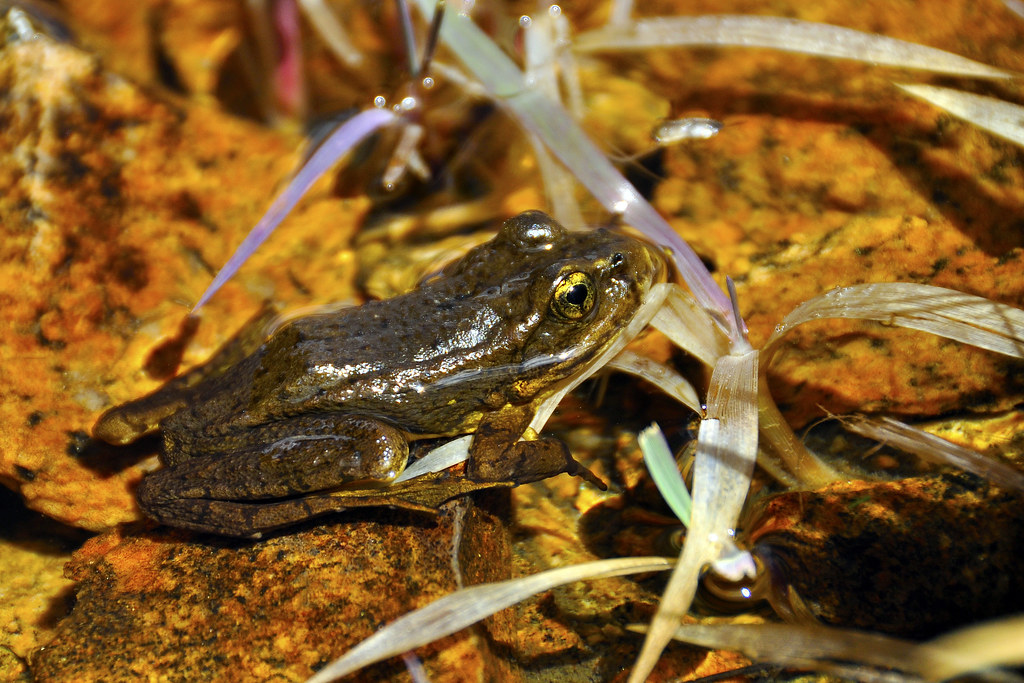
\includegraphics[width=0.4\textwidth,height=\textheight]{ylf.jpg}

Consider the following example:

Yellow-Legged frog example:\\
\emph{Population}: all yellow-legged frogs in ponds in the central
Sierra Nevada\\
\emph{Parameter}: mean body size (SVL) of adult yellow-legged frogs in
all ponds in the central Sierra Nevada\\
\emph{Sample}: As many frogs are captured and measured as possible in 10
ponds randomly sampled from the central Sierra Nevada\\
\emph{Statistic}: Sample mean

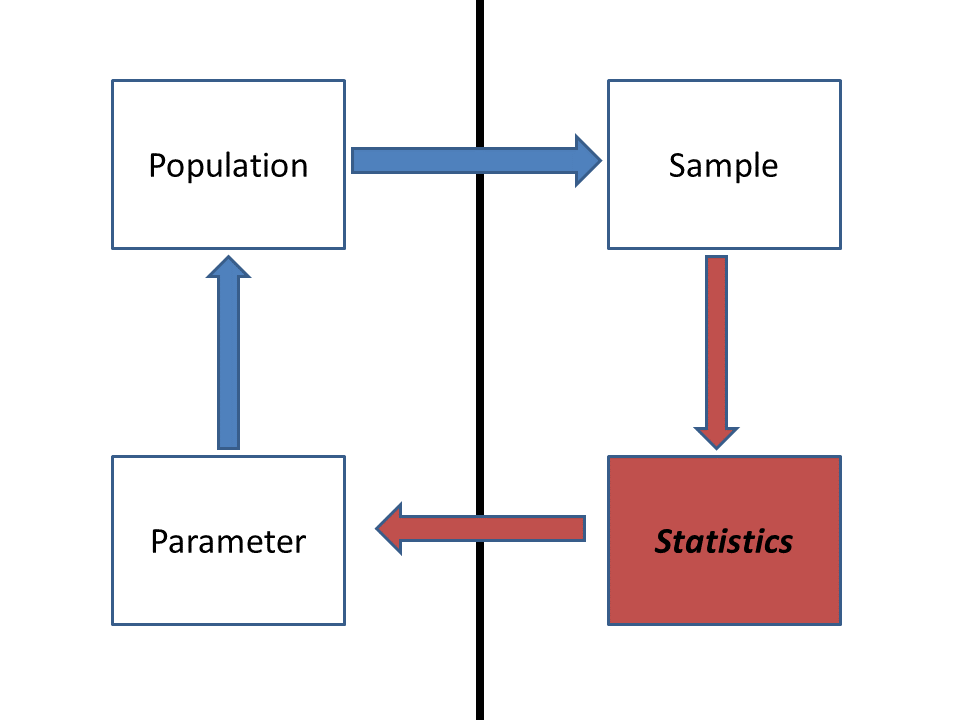
\includegraphics[width=0.4\textwidth,height=\textheight]{statistics1.png}

The goal of statistics is to infer something meaningful about a
population from a sample. In the yellow-legged frog example above, there
is a ``true'' mean body size of frogs in ponds in the central Sierra
Nevada. We just don't know what it is!

After collecting data from a sample, statistics will help us to say
something about the mean body size in the population -- both about what
we know AND what we don't know about the population!

First of all, we assume that the summary statistic computed from our
sample (n\textgreater\textgreater1) is representative of the population.
How? Why? Because of the \emph{Central Limit Theorem}.

\hypertarget{the-central-limit-theorem}{%
\subsubsection{The Central Limit
Theorem}\label{the-central-limit-theorem}}

The Central Limit Theorem (CLT) says that if you have a sample with a
reasonably large number of observations (the larger, the better!), and
each observation is independently sampled from the population, then the
statistics we compute from the sample (e.g., the sample mean) should be
reflective of the population.

For the yellow-legged frog example: our sample mean should be
representative of the mean of ALL yellow-legged frogs in the central
Sierra Nevada.

And as the sample size gets bigger, the sample mean will become more
representative of the true mean (it will converge on the true mean as
sample size approaches infinity).

The concept of \textbf{regression to the mean} is a natural consequence
of the Central Limit Theorem!

{[}In-class R demo: regression to the mean{]}

The CLT is the magic wand of statistics. It does enormous amounts of
work for us. Why?

The CLT also implies that the sampling distribution (distribution of
hypothetical samples collected from repeated sampling) for the sample
mean (and many other summary statistics) will be approximately normally
distributed -- even if the underlying data themselves are NOT normally
distributed.

Did you ever wonder why the normal (Gaussian) distribution is so common
in statistics? It's because of the CLT- many summary statistics derived
from a sample are expected to have a sampling distribution that is
\emph{approximately} normally distributed (based on the CLT)!

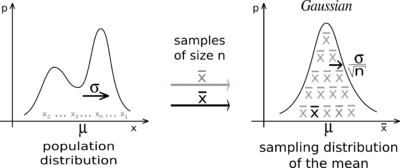
\includegraphics{clt1.png}

\hypertarget{example}{%
\subsubsection{Example}\label{example}}

How does this work? Let's use the yellow-legged frog example.

Let's say that we could measure ALL the frogs in ALL the ponds in CA.
What would that look like?

Let's simulate it using a log-normal distribution that is strongly right
skewed (positively skewed), suggesting that there are a lot of frogs out
there that are relatively small-bodied, and a few that are giants! NOTE:
this is not necessarily biologically realistic, but it makes a point.

First, let's set the population/parameter (the truth about which we hope
to make inference but can never know in reality)

\begin{Shaded}
\begin{Highlighting}[]
\CommentTok{\# Yellow{-}legged frog example {-}{-}{-}{-}{-}{-}{-}{-}{-}{-}{-}{-}{-}{-}{-}{-}{-}{-}{-}{-}{-}}

\DocumentationTok{\#\#\# ALL FROGS IN CA (the statistical population{-} all the frogs!)}

\NormalTok{allfrogs.bodysize }\OtherTok{\textless{}{-}} \FunctionTok{rlnorm}\NormalTok{(}\DecValTok{10000}\NormalTok{,}\FloatTok{1.5}\NormalTok{,}\FloatTok{0.4}\NormalTok{)        }\CommentTok{\# statistical \textquotesingle{}population\textquotesingle{}}
\FunctionTok{hist}\NormalTok{(allfrogs.bodysize,}\AttributeTok{main=}\StringTok{""}\NormalTok{,}\AttributeTok{xlab=}\StringTok{"SVL (mm)"}\NormalTok{)   }\CommentTok{\# plot out histogram}
\end{Highlighting}
\end{Shaded}

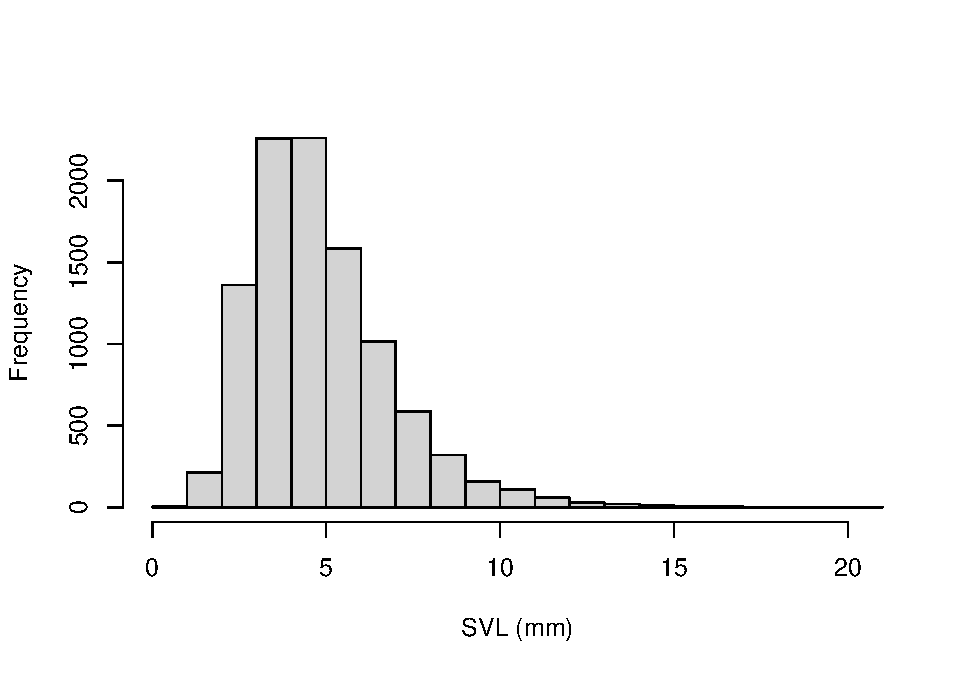
\includegraphics{LECTURE2_files/figure-latex/unnamed-chunk-3-1.pdf}

\begin{Shaded}
\begin{Highlighting}[]
\NormalTok{truemean\_SVL }\OtherTok{\textless{}{-}} \FunctionTok{mean}\NormalTok{(allfrogs.bodysize)           }\CommentTok{\# the \textquotesingle{}parameter\textquotesingle{}}
\NormalTok{truemean\_SVL }
\end{Highlighting}
\end{Shaded}

\begin{verbatim}
## [1] 4.849826
\end{verbatim}

Now let's take a sample!

\begin{Shaded}
\begin{Highlighting}[]
\NormalTok{mysample }\OtherTok{\textless{}{-}} \FunctionTok{sample}\NormalTok{(allfrogs.bodysize,}\DecValTok{10}\NormalTok{)    }\CommentTok{\# take sample of size 10 (10 frogs measured)}
\FunctionTok{mean}\NormalTok{(mysample)   }\CommentTok{\# compute the sample mean}
\end{Highlighting}
\end{Shaded}

\begin{verbatim}
## [1] 3.97039
\end{verbatim}

And another, this time with n=20

\begin{Shaded}
\begin{Highlighting}[]
\NormalTok{mysample }\OtherTok{\textless{}{-}} \FunctionTok{sample}\NormalTok{(allfrogs.bodysize,}\DecValTok{20}\NormalTok{)    }\CommentTok{\# take sample of size 20 (20 frogs measured)}
\FunctionTok{mean}\NormalTok{(mysample)   }\CommentTok{\# compute the sample mean}
\end{Highlighting}
\end{Shaded}

\begin{verbatim}
## [1] 4.64286
\end{verbatim}

Since sampling is random, sampling will produce a different result every
time.

To get a better picture of the sampling variance, let's sample many
times!

\begin{Shaded}
\begin{Highlighting}[]
\NormalTok{lotsofsamples }\OtherTok{\textless{}{-}} \FunctionTok{list}\NormalTok{()}

\ControlFlowTok{for}\NormalTok{(s }\ControlFlowTok{in} \DecValTok{1}\SpecialCharTok{:}\DecValTok{5000}\NormalTok{)\{}
\NormalTok{  lotsofsamples[[}\FunctionTok{paste0}\NormalTok{(}\StringTok{"sample"}\NormalTok{,s)]] }\OtherTok{\textless{}{-}} \FunctionTok{sample}\NormalTok{(allfrogs.bodysize,}\DecValTok{30}\NormalTok{)    }\CommentTok{\# take sample of size 30 (30 frogs measured)}
\NormalTok{\}}

\NormalTok{lotsofsamples}\SpecialCharTok{$}\NormalTok{sample1}
\end{Highlighting}
\end{Shaded}

\begin{verbatim}
##  [1]  4.712516  5.251493  3.128509  7.942776  4.767070  4.599820  4.177680  4.553496  3.963093  4.359347
## [11]  3.352357  8.247807  2.678960  4.961782  9.592330  8.047735  7.763867  5.287346 10.504452  6.421929
## [21]  4.376636  2.880076  3.954936  3.824857  2.179980  6.904980  5.607723  4.125540  3.862737  4.179014
\end{verbatim}

\begin{Shaded}
\begin{Highlighting}[]
\NormalTok{lotsofsamples}\SpecialCharTok{$}\NormalTok{sample99}
\end{Highlighting}
\end{Shaded}

\begin{verbatim}
##  [1]  6.025209  5.879259 10.413671  4.014657  2.758221  5.742516  1.703173  3.892715  4.550972  3.962358
## [11]  2.446267  3.594997  4.740672  6.633364  8.256432  2.617211  4.199229  4.176399  6.151317  6.516149
## [21]  3.761666  7.936469  3.833904  4.613205  2.004393  4.019660  6.169324  5.635727  5.543839  6.395076
\end{verbatim}

\begin{Shaded}
\begin{Highlighting}[]
\NormalTok{lotsofsamples}\SpecialCharTok{$}\NormalTok{sample732}
\end{Highlighting}
\end{Shaded}

\begin{verbatim}
##  [1]  4.398425  7.727090  9.552409  5.161039  3.513062  3.418455  3.956433 10.650780  3.974201  5.821207
## [11]  2.209968  4.125540  3.462340  3.641449  5.968085  4.521117  4.207564  4.702996  5.928669  5.425030
## [21]  5.561796  4.208950  2.081193  2.605480  2.268815  5.050107  4.011845  3.081823  3.912276  4.007705
\end{verbatim}

Now we can compute the sample means and the sampling variance for the
summary statistic (mean body size)

\begin{Shaded}
\begin{Highlighting}[]
\NormalTok{samplemeans }\OtherTok{\textless{}{-}} \FunctionTok{sapply}\NormalTok{(lotsofsamples,mean)}

\FunctionTok{hist}\NormalTok{(samplemeans,}\AttributeTok{xlab=}\StringTok{"mean body size (n=30)"}\NormalTok{)    }\CommentTok{\# visualize the sampling distribution!}
\end{Highlighting}
\end{Shaded}

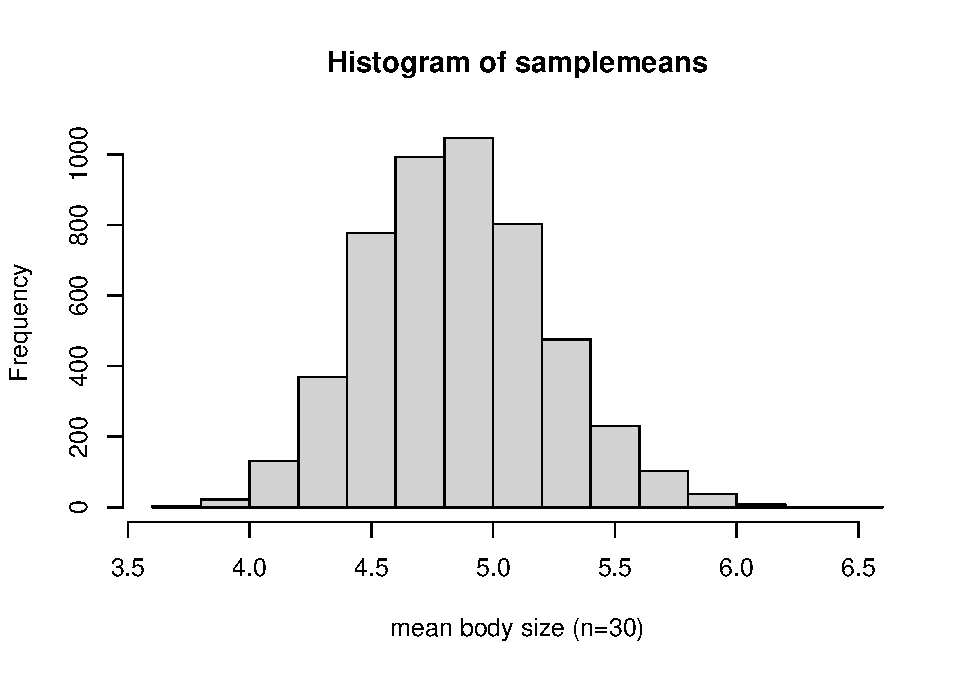
\includegraphics{LECTURE2_files/figure-latex/unnamed-chunk-7-1.pdf}

Interesting- does this look skewed to you? Doesn't it look like a normal
distribution??

It's the CLT at work!!

Of all the samples you could get, there are very few that are all at one
end of the distribution. There are a lot more possible random samples
that span the full distribution of values, from low to high. Take the
average af all those values, low and high, and you get something in the
middle. The normal distribution is humped right in the middle, because
of the tendency for low and high observations to `average out' within a
sample.

\hypertarget{coin-flipping-example}{%
\subsubsection{Coin flipping example}\label{coin-flipping-example}}

Here's the sampling distribution for the number of heads out of a single
coin flip (either 0 or 1!):

\begin{Shaded}
\begin{Highlighting}[]
\FunctionTok{barplot}\NormalTok{(}\FunctionTok{table}\NormalTok{(}\FunctionTok{rbinom}\NormalTok{(}\DecValTok{10000}\NormalTok{,}\DecValTok{1}\NormalTok{,.}\DecValTok{5}\NormalTok{))}\SpecialCharTok{/}\DecValTok{10000}\NormalTok{,}\AttributeTok{xlab=}\StringTok{"N heads out of 1"}\NormalTok{,}\AttributeTok{ylab=}\StringTok{"Probability"}\NormalTok{)}
\end{Highlighting}
\end{Shaded}

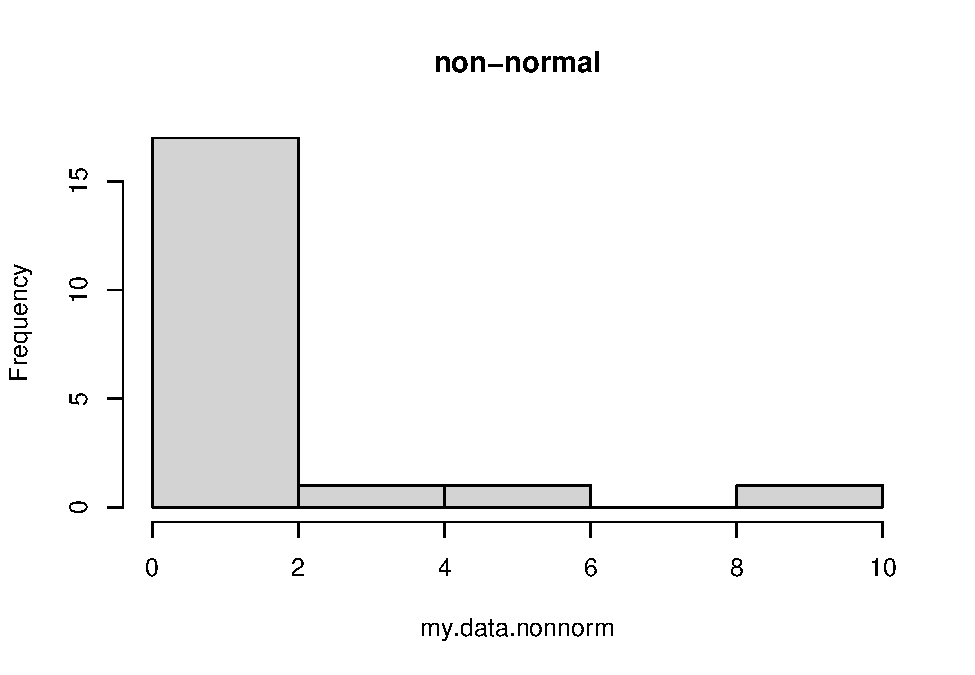
\includegraphics{LECTURE2_files/figure-latex/unnamed-chunk-8-1.pdf}

Now let's build up sample size and see how the sampling distribution
changes.

\begin{Shaded}
\begin{Highlighting}[]
\FunctionTok{par}\NormalTok{(}\AttributeTok{mfrow=}\FunctionTok{c}\NormalTok{(}\DecValTok{3}\NormalTok{,}\DecValTok{2}\NormalTok{))}
\ControlFlowTok{for}\NormalTok{(i }\ControlFlowTok{in} \FunctionTok{seq}\NormalTok{(}\DecValTok{2}\NormalTok{,}\DecValTok{12}\NormalTok{,}\DecValTok{2}\NormalTok{))\{}
   \FunctionTok{barplot}\NormalTok{(}\FunctionTok{table}\NormalTok{(}\FunctionTok{rbinom}\NormalTok{(}\DecValTok{10000}\NormalTok{,i,.}\DecValTok{5}\NormalTok{))}\SpecialCharTok{/}\DecValTok{10000}\NormalTok{,}\AttributeTok{xlab=}\FunctionTok{sprintf}\NormalTok{(}\StringTok{"N heads out of \%s"}\NormalTok{,i),}\AttributeTok{ylab=}\StringTok{"Probability"}\NormalTok{,}\AttributeTok{main=}\FunctionTok{paste0}\NormalTok{(}\StringTok{"sample size = "}\NormalTok{,i))}
   \CommentTok{\#hist(rbinom(10000,i,.5),main=paste0("sample size = ",i),xlab=sprintf("N heads out of \%s",i)) }
\NormalTok{\}}
\end{Highlighting}
\end{Shaded}

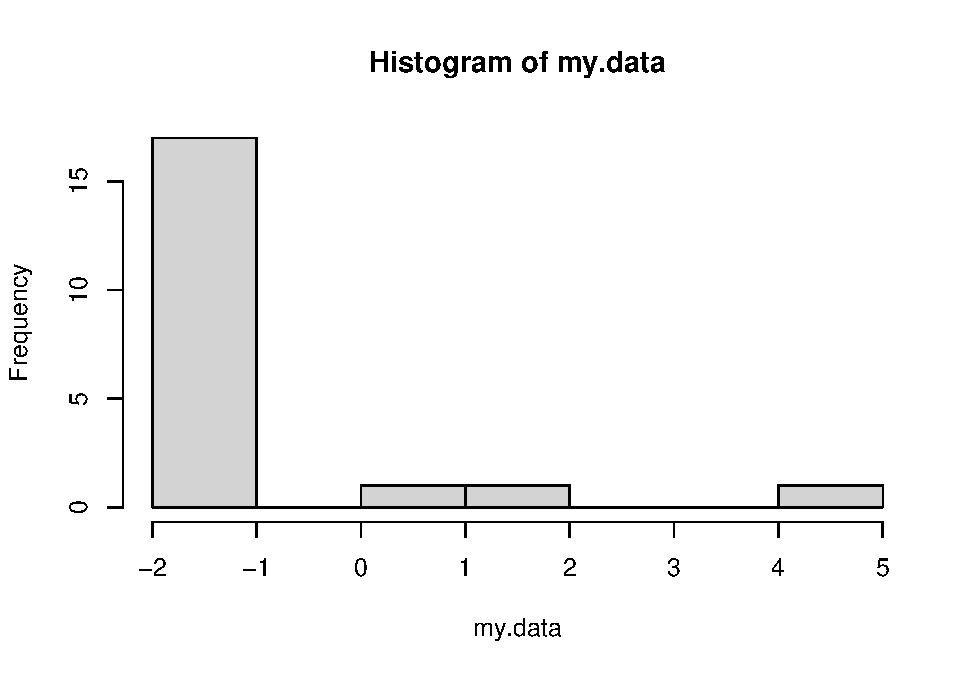
\includegraphics{LECTURE2_files/figure-latex/unnamed-chunk-9-1.pdf}

And with really big sample size:

\begin{Shaded}
\begin{Highlighting}[]
\FunctionTok{hist}\NormalTok{(}\FunctionTok{rbinom}\NormalTok{(}\DecValTok{10000}\NormalTok{,}\DecValTok{1000}\NormalTok{,.}\DecValTok{5}\NormalTok{),}\AttributeTok{xlab=}\StringTok{"N heads out of 1000"}\NormalTok{,}\AttributeTok{freq =}\NormalTok{ F, }\AttributeTok{main=}\StringTok{""}\NormalTok{)}
\end{Highlighting}
\end{Shaded}

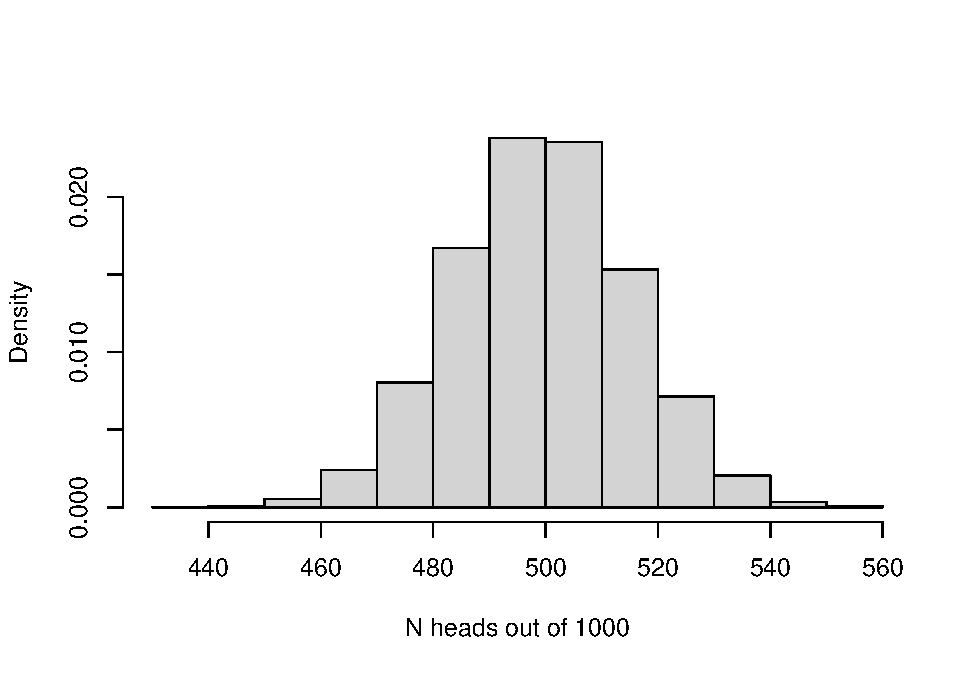
\includegraphics{LECTURE2_files/figure-latex/unnamed-chunk-10-1.pdf}

The larger the sample size, the more closely the sampling distribution
(number of heads out of N flips of a fair coin) looks like a normal
distribution! Again, the CLT at work!

\hypertarget{sampling-distributions-in-null-hypothesis-testing}{%
\subsection{Sampling distributions in null hypothesis
testing}\label{sampling-distributions-in-null-hypothesis-testing}}

Pretty much all of classical null hypothesis testing (NHT) works like
this:

\begin{enumerate}
\def\labelenumi{\arabic{enumi}.}
\tightlist
\item
  We compute a summary statistic from our data. This statistic
  represents the ``signal'' in your data.\\
\item
  Using the known (theoretical) sampling distribution for our summary
  statistic under the null hypothesis (worked out by statisticians!), we
  inquire whether or not our summary statistic (signal) could have been
  a result of random sampling error under the null hypothesis.
\item
  If it is implausble that random noise could have produced our result
  (if \(p\le\alpha\)) then we reject the null hypothesis. Otherwise we
  fail to reject the null\ldots{}
\end{enumerate}

Sampling distributions that are commonly used include:

\begin{itemize}
\tightlist
\item
  t distribution (sampling distribution for the t statistic under the
  null hypothesis)
\item
  z distribution (assume your test statistic is a standard normal
  distribution)
\item
  Chi-squared distribution (sampling distribution for the Chi-squared
  statistic under the null hypothesis)
\item
  F distribution (sampling distribution for the F statistic under the
  null hypothesis- used in ANOVA and regression)
\end{itemize}

Sampling distributions are thought experiments! What would our test
statistic look like under repeated sampling from a population (e.g.,
under the null hypothesis)?

\hypertarget{summary-metrics-calculated-from-sample-data}{%
\subsection{Summary metrics (calculated from sample
data)}\label{summary-metrics-calculated-from-sample-data}}

We often summarize our samples by their centers (e.g., average) and
their spread (dispersion). These informative data summaries are useful
on their own, and are also used to compute statistics like the t or F
statistics.

\hypertarget{center-statistics-means-medians-geometric-mean}{%
\subsubsection{``Center'' statistics: means, medians, geometric
mean}\label{center-statistics-means-medians-geometric-mean}}

Sample Mean (arithmetic mean) = sum of all sampled values divided by the
sample size\\
Sample Median (midway point) = 50\% quantile. Order the values and
select the value at the center.

Sample Geometric mean: product of numbers taken to the nth root. For two
numbers, 3 and 4, you'd have the sq root of 3*4 = 3.46

\hypertarget{data-spread-or-dispersion}{%
\subsubsection{Data spread, or
dispersion:}\label{data-spread-or-dispersion}}

Standard deviations and variances are calculated differently depending
on whether we are computing these quantities for an entire population of
interest vs a sample drawn from a larger population!

Standard Deviation -- sigma (\(\sigma\)) for population standard
deviation, \emph{s} for the sample standard deviation.

Variance- (\(\sigma^2\)) for population variance, (\(s^2\)) for the
sample variance

The variance represents the average squared difference from the mean.
The standard deviation represents the square root of the variance.

Standard deviation is much more commonly reported than variance because
it is in the same units/scale as the original measurements.

Coefficient of variation (cv) is the standard deviation represented as a
fraction of the mean.

\hypertarget{variance-and-std-deviation-calculation-example}{%
\paragraph{Variance and Std deviation calculation
example}\label{variance-and-std-deviation-calculation-example}}

For a population:
\(\sigma = \sqrt{\sum_{n=1}^{i}{\frac{(x_i-\mu)^2}{N}}}\)

For example: compute the variance of 5 numbers: 4, 3, 5, 5, 2

\(\mu = (4+3+5+5+2)/5 = 3.8\)

(4-3.8)\^{}2 = 0.2\^{}2 = 0.04\\
(3-3.8)\^{}2 = 0.64\\
(5-3.8)\^{}2 = 1.44\\
(5-3.8)\^{}2 = 1.44\\
(2-3.8)\^{}2 = 3.24

Sum these = 6.8\\
Divide by 5 = population variance = 6.8/5 = 1.36 Take square root =
\(\sigma\) = 1.17

For a sample (estimating population variance from a sample):
\(s = \sqrt{\sum_{n=1}^{i}{\frac{(x_i-\bar{x})^2}{(N-1)}}}\)

\(\bar{x} = (4+3+5+5+2)/5 = 3.8\)

(4-3.8)\^{}2 = 0.2\^{}2 = 0.04\\
(3-3.8)\^{}2 = 0.64\\
(5-3.8)\^{}2 = 1.44\\
(5-3.8)\^{}2 = 1.44\\
(2-3.8)\^{}2 = 3.24

Sum these = 6.8\\
Divide by 4 = sample variance = 6.8/4 = 1.7\\
Take square root = \(s\) = 1.30

So the population sd is 1.36 whereas the sample sd is 1.7.

\hypertarget{aside-degrees-of-freedom}{%
\paragraph{Aside: degrees of freedom}\label{aside-degrees-of-freedom}}

OK, so why the different estimates of dispersion for population
vs.~sample?

Which is larger? Which are we less confident in?

This has to do with a concept called \emph{degrees of freedom}.

Sigma can be computed with 100\% accuracy. Since you have the entire
population measured, you can compute a measure of dispersion for the
population and that measure is perfect. It is not an estimate.

The sample standard deviation \(s\), on the other hand, is an imperfect
estimate of dispersion for a much larger population! In fact, if we used
the population formula for a sample, it would underestimate the
dispersion of the target population.

Th reason for this is that the formula for sample stdev \emph{uses the
sample mean}, not the population mean. In fact, the same sample data
were used to compute the sample mean! If you know the values of four of
the five sampled values AND we know that the sample mean, we know what
the value of the final observation must be. Therefore, even though we
have 5 data points, we have only 4 \emph{degrees of freedom} if the
sample mean is included in our formula. In this case, we have four
independent pieces of information that we can use for computing standard
deviation (we `spent' one degree of freedom already to compute the
sample mean!).

By dividing the sum of squared deviations from the sample mean by 4
instead of 5, we are \emph{unbiasing} the estimate of dispersion to
account for the fact that we are using the sample data twice- once for
computing the mean, next for computing the standard deviation!

\hypertarget{sampling-distributions}{%
\subsection{Sampling distributions}\label{sampling-distributions}}

Statisticians worked out the sampling distributions (often called the
sampling variance- don't confuse this with the `sample variance' we
discussed above!) for some common summary statistics.

\hypertarget{standard-error-of-the-mean}{%
\subsubsection{Standard error of the
mean}\label{standard-error-of-the-mean}}

Standard error of the mean = sample std deviation divided by the square
root of the sample size

\(se = \frac{s}{\sqrt{N}}\)

The standard error of the mean is used to help us describe the sampling
distribution for the sample mean (the expected distribution of sample
means if you collected thousands of new samples and computed the mean).

\begin{Shaded}
\begin{Highlighting}[]
\CommentTok{\# Survey of common sampling distributions {-}{-}{-}{-}{-}{-}{-}{-}{-}{-}{-}{-}{-}{-}{-}{-}{-}}

\CommentTok{\# Sampling distribution: the sample mean}

\NormalTok{mysample }\OtherTok{\textless{}{-}} \FunctionTok{c}\NormalTok{(}\FloatTok{4.1}\NormalTok{,}\FloatTok{3.5}\NormalTok{,}\FloatTok{3.7}\NormalTok{,}\FloatTok{6.6}\NormalTok{,}\FloatTok{8.0}\NormalTok{,}\FloatTok{5.4}\NormalTok{,}\FloatTok{7.3}\NormalTok{,}\FloatTok{4.4}\NormalTok{)}
\NormalTok{mysample}
\end{Highlighting}
\end{Shaded}

\begin{verbatim}
## [1] 4.1 3.5 3.7 6.6 8.0 5.4 7.3 4.4
\end{verbatim}

\begin{Shaded}
\begin{Highlighting}[]
\NormalTok{n }\OtherTok{\textless{}{-}} \FunctionTok{length}\NormalTok{(mysample)    }\CommentTok{\# sample size}
\NormalTok{sample.mean }\OtherTok{\textless{}{-}} \FunctionTok{mean}\NormalTok{(mysample)  }\CommentTok{\# sample mean}
\NormalTok{sample.stdev }\OtherTok{\textless{}{-}} \FunctionTok{sd}\NormalTok{(mysample)   }\CommentTok{\# sample standard deviation (r uses denominator of n{-}1 by default!)}
\NormalTok{std.error }\OtherTok{\textless{}{-}}\NormalTok{ sample.stdev}\SpecialCharTok{/}\FunctionTok{sqrt}\NormalTok{(n) }

\NormalTok{std.error }
\end{Highlighting}
\end{Shaded}

\begin{verbatim}
## [1] 0.6122995
\end{verbatim}

Now we have all the information we need to compute the sampling
distribution for the sample mean.

Our sample mean is 5.375. But if we collected different samples of size
n=8, we would get different values - even if the true population mean
was 5.375. What does this distribution of values look like?

\begin{Shaded}
\begin{Highlighting}[]
\NormalTok{sampdist }\OtherTok{\textless{}{-}} \ControlFlowTok{function}\NormalTok{(x)\{}\FunctionTok{dt}\NormalTok{((x}\SpecialCharTok{{-}}\NormalTok{sample.mean)}\SpecialCharTok{/}\NormalTok{std.error,n}\DecValTok{{-}1}\NormalTok{)\}}
\FunctionTok{curve}\NormalTok{(sampdist,}\DecValTok{0}\NormalTok{,}\DecValTok{11}\NormalTok{,}\AttributeTok{ylab=}\StringTok{"probability density"}\NormalTok{,}\AttributeTok{xlab=}\StringTok{"value"}\NormalTok{,}\AttributeTok{main=}\StringTok{"sampling distribution for the sample mean!"}\NormalTok{)}
\FunctionTok{abline}\NormalTok{(}\AttributeTok{v=}\NormalTok{sample.mean,}\AttributeTok{col=}\StringTok{"green"}\NormalTok{,}\AttributeTok{lwd=}\DecValTok{3}\NormalTok{)}
\NormalTok{confint }\OtherTok{\textless{}{-}} \FunctionTok{c}\NormalTok{(sample.mean}\SpecialCharTok{+}\NormalTok{std.error}\SpecialCharTok{*}\FunctionTok{qt}\NormalTok{(}\FloatTok{0.025}\NormalTok{,n}\DecValTok{{-}1}\NormalTok{),sample.mean}\SpecialCharTok{+}\NormalTok{std.error}\SpecialCharTok{*}\FunctionTok{qt}\NormalTok{(}\FloatTok{0.975}\NormalTok{,n}\DecValTok{{-}1}\NormalTok{))}
\FunctionTok{abline}\NormalTok{(}\AttributeTok{v=}\NormalTok{confint,}\AttributeTok{col=}\StringTok{"blue"}\NormalTok{,}\AttributeTok{lty=}\DecValTok{2}\NormalTok{)}
\end{Highlighting}
\end{Shaded}

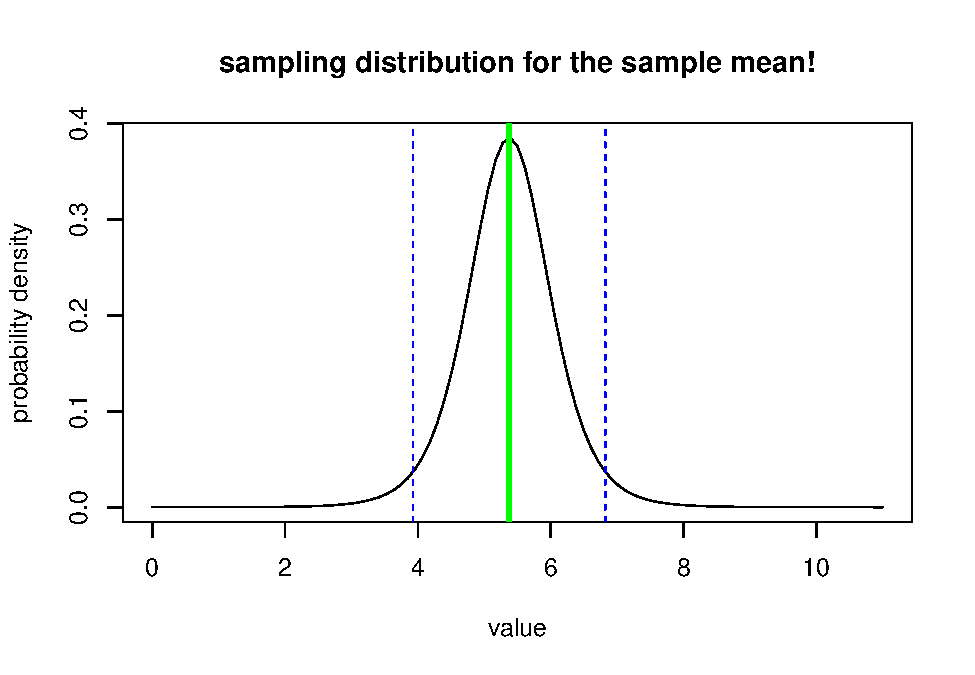
\includegraphics{LECTURE2_files/figure-latex/unnamed-chunk-12-1.pdf}

The vertical blue lines indicate the \emph{confidence interval} around
the mean with the \emph{confidence level} set at 95\% - the confidence
interval helps us visualize what might happen if we repeated our
sampling over and over and over- how might our result change?

Note the use of the \emph{t distribution} in the above code block. The t
distribution is a theoretical sampling distribution representing
sampling error in units of standard error.

\hypertarget{confidence-intervals}{%
\subsubsection{Confidence intervals}\label{confidence-intervals}}

Confidence intervals, like p-values, are commonly misinterpreted!

In classical frequentist statistics, the population parameter of
interest is fixed- there is no uncertainty associated with the
population parameter itself -- it's just that we can only collect and
assess a small sample from the much larger population. So it does not
make sense to say something like ``the true parameter has a 90\% chance
of falling within the confidence interval''. The true parameter is
either in the interval or it is not in the interval. All we can say is
something more like ``90\% of confidence intervals generated from
different random samples would contain the true parameter''.

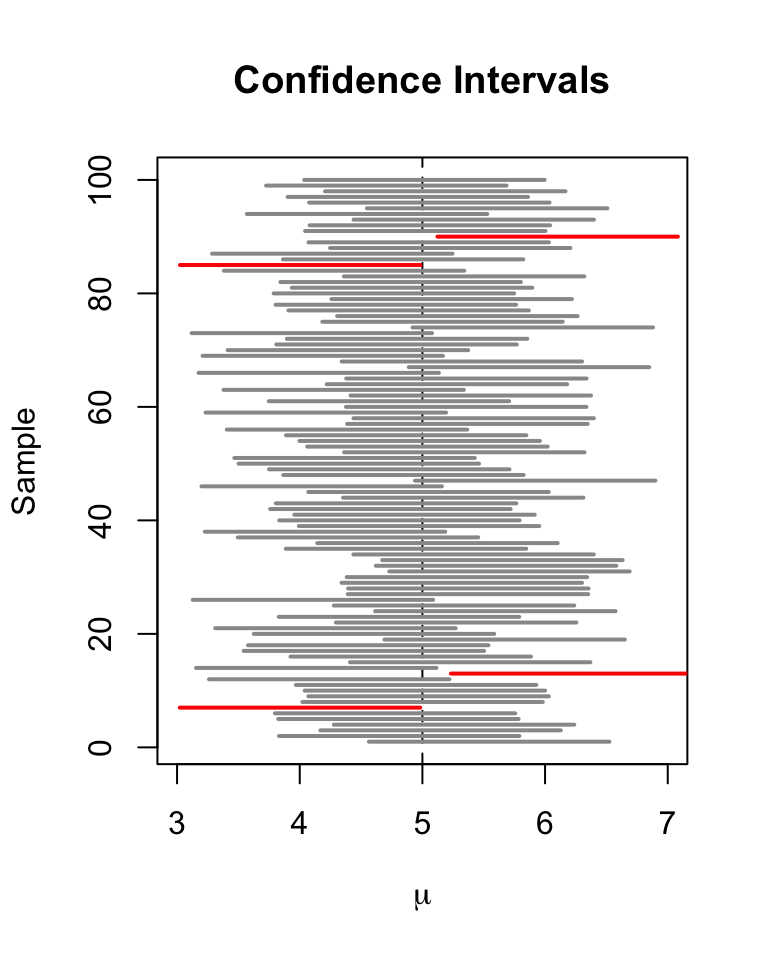
\includegraphics[width=0.4\textwidth,height=\textheight]{confint1.png}

We unfortunately have no idea if our particular confidence interval is
one that includes the true parameter, or one that does not!!

Don't worry if you find this difficulty- everyone does! And practically
speaking, just about everyone interprets a 95\% confidence interval as
having a 95\% probability of including the true parameter - and it
doesn't really matter that much!

\hypertarget{probability-distributions--the-basics-and-how-to-use-them-in-r}{%
\subsection{Probability distributions- the basics (and how to use them
in
R)}\label{probability-distributions--the-basics-and-how-to-use-them-in-r}}

\hypertarget{discrete-vs.-continuous}{%
\subsubsection{Discrete vs.~continuous}\label{discrete-vs.-continuous}}

In \emph{discrete distributions}, each outcome (value that could be
sampled under this probability distribution) has a specific
\emph{probability mass} (like the probability of flipping a coin 10
times and getting 4 heads). For example, let's consider the Poisson
distribution:

\begin{Shaded}
\begin{Highlighting}[]
\CommentTok{\# Probability distributions {-}{-}{-}{-}{-}{-}{-}{-}{-}{-}{-}{-}{-}{-}{-}{-}{-}{-}{-}{-}{-}}

\CommentTok{\# Discrete probability distributions }

\NormalTok{mean }\OtherTok{\textless{}{-}} \DecValTok{5}
\FunctionTok{rpois}\NormalTok{(}\DecValTok{10}\NormalTok{,mean)    }\CommentTok{\# note: the random numbers sampled from this distribution have no decimal component}
\end{Highlighting}
\end{Shaded}

\begin{verbatim}
##  [1] 6 8 4 3 4 3 2 6 5 4
\end{verbatim}

\begin{Shaded}
\begin{Highlighting}[]
             \CommentTok{\# plot discrete probabilities of getting particular outcomes!}
\NormalTok{xvals }\OtherTok{\textless{}{-}} \FunctionTok{seq}\NormalTok{(}\DecValTok{0}\NormalTok{,}\DecValTok{15}\NormalTok{,}\DecValTok{1}\NormalTok{)}
\NormalTok{probs }\OtherTok{\textless{}{-}} \FunctionTok{dpois}\NormalTok{(xvals,}\AttributeTok{lambda=}\NormalTok{mean)}
\FunctionTok{names}\NormalTok{(probs) }\OtherTok{\textless{}{-}}\NormalTok{ xvals}
               
\FunctionTok{barplot}\NormalTok{(probs,}\AttributeTok{ylab=}\StringTok{"Probability Mass"}\NormalTok{,}\AttributeTok{main=}\StringTok{"Poisson distribution (discrete)"}\NormalTok{)}
\end{Highlighting}
\end{Shaded}

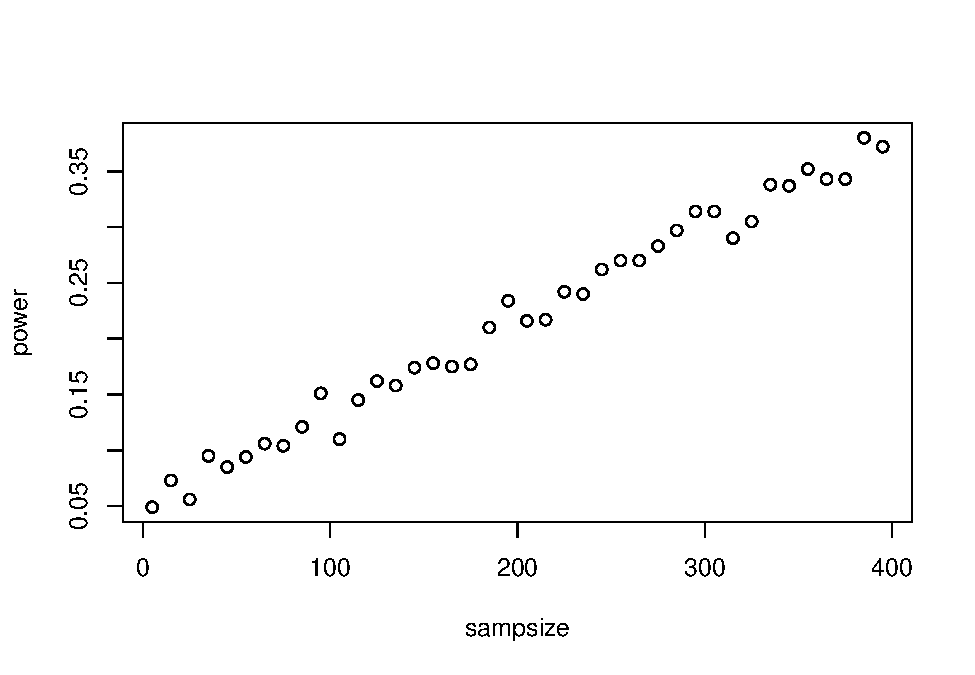
\includegraphics{LECTURE2_files/figure-latex/unnamed-chunk-13-1.pdf}

\begin{Shaded}
\begin{Highlighting}[]
\FunctionTok{barplot}\NormalTok{(}\FunctionTok{cumsum}\NormalTok{(probs),}\AttributeTok{ylab=}\StringTok{"Cumulative Probability"}\NormalTok{,}\AttributeTok{main=}\StringTok{"Poisson distribution (discrete)"}\NormalTok{)   }\CommentTok{\# cumulative distribution}
\end{Highlighting}
\end{Shaded}

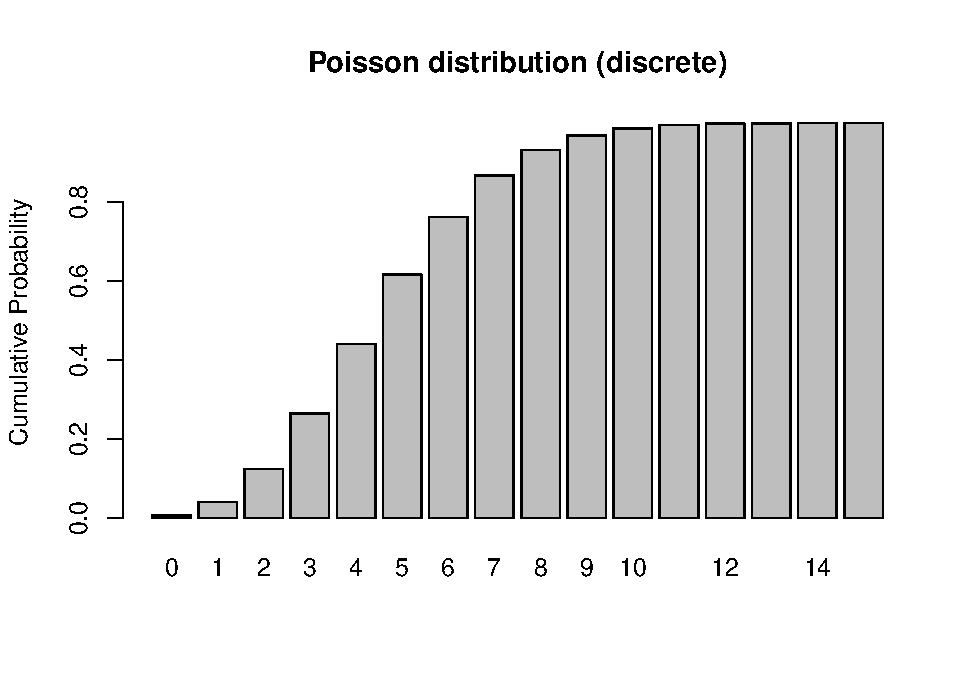
\includegraphics{LECTURE2_files/figure-latex/unnamed-chunk-13-2.pdf}

\begin{Shaded}
\begin{Highlighting}[]
\FunctionTok{sum}\NormalTok{(probs)   }\CommentTok{\# just to make sure it sums to 1!  Does it???}
\end{Highlighting}
\end{Shaded}

\begin{verbatim}
## [1] 0.999931
\end{verbatim}

In \emph{continuous distributions}, each possible value/quantity that
could be randomly sampled is associated with a \emph{probability
density}, \(f(x)\), not probability mass \(Prob(x)\). This is because
the probability of getting any particular value in a continuous
distribution is effectively zero. This arises from the problem of
precision. The sum of the probability distribution must be 1 (there is
only 100\% of probability to go around). In a continuous distribution,
there are an infinite number of possible values of x. So any individual
probability is always divided by infinity, which makes it zero.
Therefore we have to talk about probability density, unless we want to
specify a particular range of values -- we can't calculate
\(Prob(x = 5)\), but we can calculate \(Prob(4 < x < 6)\) or
\(Prob(x > 5)\). The probability density is defined as the probability
of getting a value within an infinitesimally small range of a particular
value, divided by that infinitesimally small interval. No worries if you
don't understand that - you can just think of probability density as the
relative likelihood of sampling one value versus another. Let's consider
the beta distribution:

\begin{Shaded}
\begin{Highlighting}[]
\CommentTok{\# continuous distributions}

\NormalTok{shape1 }\OtherTok{=} \FloatTok{0.5}
\NormalTok{shape2 }\OtherTok{=} \FloatTok{0.5}

\FunctionTok{rbeta}\NormalTok{(}\DecValTok{10}\NormalTok{,shape1,shape2)   }\CommentTok{\# generate 10 random numbers from a continuous distribution}
\end{Highlighting}
\end{Shaded}

\begin{verbatim}
##  [1] 9.385631e-01 1.085078e-01 2.051230e-01 3.262719e-06 9.234675e-02 6.265471e-01 8.333576e-01 8.686447e-01
##  [9] 4.201532e-01 8.467183e-01
\end{verbatim}

\begin{Shaded}
\begin{Highlighting}[]
\FunctionTok{curve}\NormalTok{(}\FunctionTok{dbeta}\NormalTok{(x,shape1,shape2),}\AttributeTok{ylab=}\StringTok{"probability density"}\NormalTok{,}\AttributeTok{xlab=}\StringTok{"possibilities"}\NormalTok{)   }\CommentTok{\# probability density function (PDF)}
\end{Highlighting}
\end{Shaded}

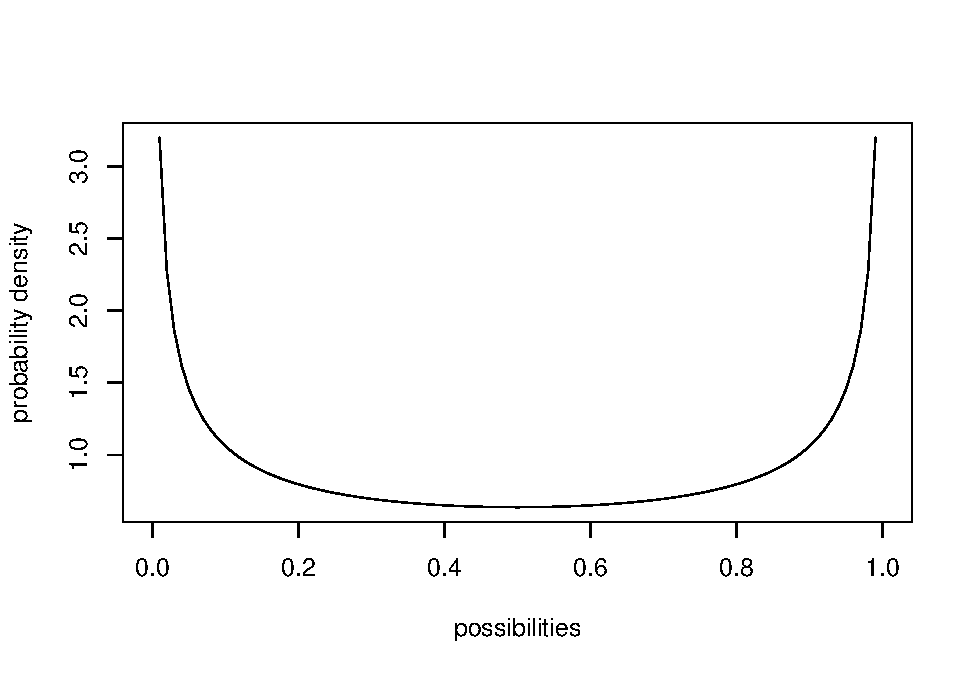
\includegraphics{LECTURE2_files/figure-latex/unnamed-chunk-14-1.pdf}

\begin{Shaded}
\begin{Highlighting}[]
\FunctionTok{curve}\NormalTok{(}\FunctionTok{pbeta}\NormalTok{(x,shape1,shape2),}\AttributeTok{ylab=}\StringTok{"cumulative probability"}\NormalTok{,}\AttributeTok{xlab=}\StringTok{"possibilities"}\NormalTok{)   }\CommentTok{\# cumulative distribution}
\end{Highlighting}
\end{Shaded}

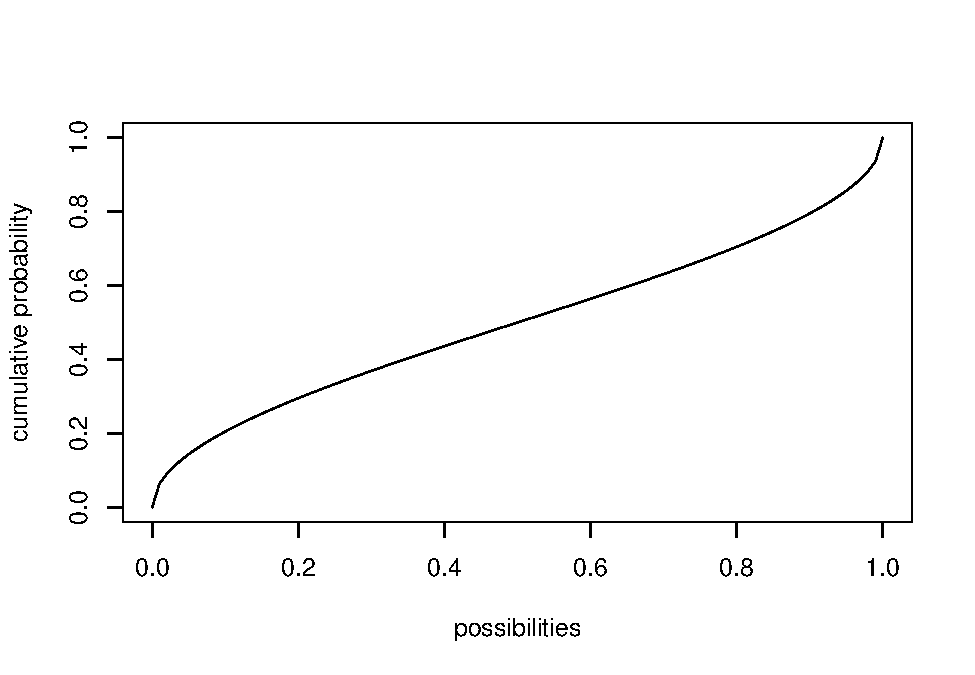
\includegraphics{LECTURE2_files/figure-latex/unnamed-chunk-14-2.pdf}

\begin{Shaded}
\begin{Highlighting}[]
\FunctionTok{integrate}\NormalTok{(}\AttributeTok{f=}\NormalTok{dbeta,}\AttributeTok{lower=}\DecValTok{0}\NormalTok{,}\AttributeTok{upper=}\DecValTok{1}\NormalTok{,}\AttributeTok{shape1=}\NormalTok{shape1,}\AttributeTok{shape2=}\NormalTok{shape2)    }\CommentTok{\# just to make sure it integrates to 1!!}
\end{Highlighting}
\end{Shaded}

\begin{verbatim}
## 1 with absolute error < 3e-06
\end{verbatim}

\hypertarget{probability-distributions-in-r}{%
\subsubsection{Probability distributions in
R}\label{probability-distributions-in-r}}

\hypertarget{random-number-generators}{%
\paragraph{Random number generators}\label{random-number-generators}}

\textbf{Random number generators} are functions for generating random
values from a specified probability distribution (e.g., `rnorm',
`rpois', `rt')

\begin{Shaded}
\begin{Highlighting}[]
\CommentTok{\# random number generators}

\FunctionTok{rnorm}\NormalTok{(}\DecValTok{10}\NormalTok{)    }\CommentTok{\# generate 10 random numbers from a standard normal distribution}
\end{Highlighting}
\end{Shaded}

\begin{verbatim}
##  [1]  1.81545134  1.40187273 -0.39124208 -1.80531407 -0.96309109 -1.59639569  0.97336657 -0.31185089
##  [9]  0.42543491  0.01808547
\end{verbatim}

\begin{Shaded}
\begin{Highlighting}[]
\FunctionTok{rnorm}\NormalTok{(}\DecValTok{5}\NormalTok{,}\DecValTok{25}\NormalTok{,}\DecValTok{5}\NormalTok{)  }\CommentTok{\# generate 5 random numbers from a normal distribution with mean=25 and sd=5}
\end{Highlighting}
\end{Shaded}

\begin{verbatim}
## [1] 24.77623 23.45544 19.78327 27.30770 22.59897
\end{verbatim}

\begin{Shaded}
\begin{Highlighting}[]
\FunctionTok{rpois}\NormalTok{(}\DecValTok{8}\NormalTok{,}\DecValTok{18}\NormalTok{)  }\CommentTok{\# generate 8 random numbers from a poisson distribution with mean=18}
\end{Highlighting}
\end{Shaded}

\begin{verbatim}
## [1] 19 17 26 12 15 22 17 20
\end{verbatim}

\hypertarget{probability-density-functions}{%
\paragraph{Probability density
functions}\label{probability-density-functions}}

Continuous distributions are associated with \textbf{PDFs}, or
probability density functions (e.g., `dnorm',`dt',`dgamma'). These
functions give you the probability density (relative probability) of any
particular value/quantity that could be randomly sampled under this
distribution.

\begin{Shaded}
\begin{Highlighting}[]
\DocumentationTok{\#\# probability density function example }

\FunctionTok{curve}\NormalTok{(}\FunctionTok{dt}\NormalTok{(x,}\DecValTok{8}\NormalTok{),}\SpecialCharTok{{-}}\DecValTok{4}\NormalTok{,}\DecValTok{4}\NormalTok{,}\AttributeTok{xlab=}\StringTok{"possibilities"}\NormalTok{,}\AttributeTok{ylab=}\StringTok{\textquotesingle{}relative probability (prob density)\textquotesingle{}}\NormalTok{)}
\end{Highlighting}
\end{Shaded}

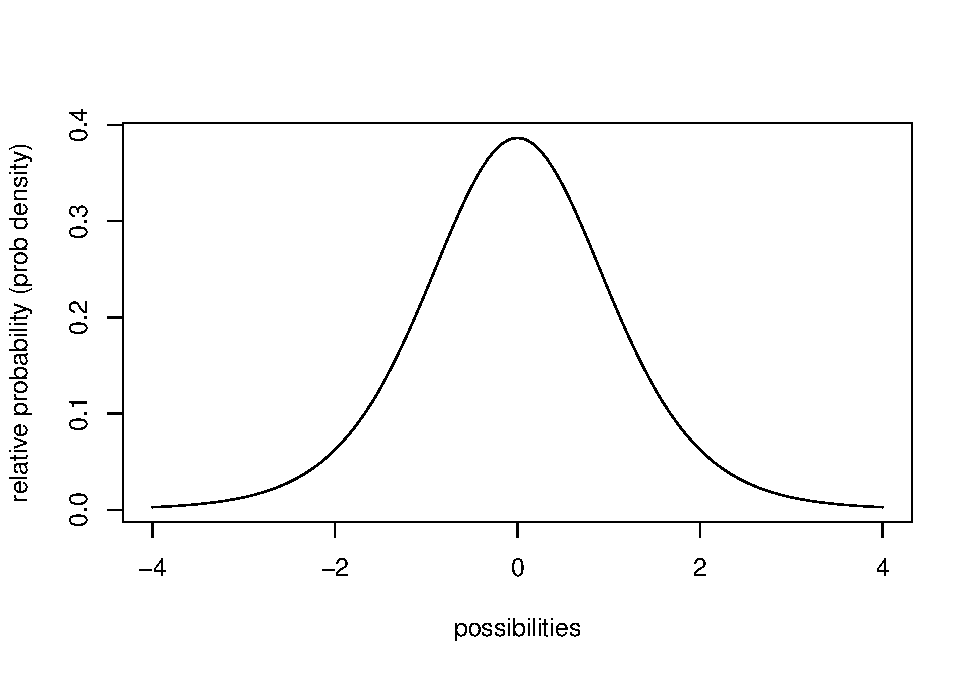
\includegraphics{LECTURE2_files/figure-latex/unnamed-chunk-16-1.pdf}

\hypertarget{probability-mass-functions}{%
\paragraph{Probability mass
functions}\label{probability-mass-functions}}

For discrete distributions, \textbf{PMFs} - Probability mass functions
(e.g., `dpois',`dbinom') -- give you the exact probability of obtaining
any particular value that could be sampled under this distribution.

\begin{Shaded}
\begin{Highlighting}[]
\DocumentationTok{\#\# probability mass function example }

\NormalTok{x }\OtherTok{\textless{}{-}} \FunctionTok{barplot}\NormalTok{(}\FunctionTok{sapply}\NormalTok{(}\DecValTok{0}\SpecialCharTok{:}\DecValTok{10}\NormalTok{,}\ControlFlowTok{function}\NormalTok{(t) }\FunctionTok{dpois}\NormalTok{(t,}\DecValTok{2}\NormalTok{)),}\AttributeTok{xlab=}\StringTok{"possibilities"}\NormalTok{,}\AttributeTok{ylab=}\StringTok{\textquotesingle{}probability\textquotesingle{}}\NormalTok{)}
\FunctionTok{axis}\NormalTok{(}\DecValTok{1}\NormalTok{,}\AttributeTok{at=}\NormalTok{x,}\AttributeTok{labels=}\DecValTok{0}\SpecialCharTok{:}\DecValTok{10}\NormalTok{)}
\end{Highlighting}
\end{Shaded}

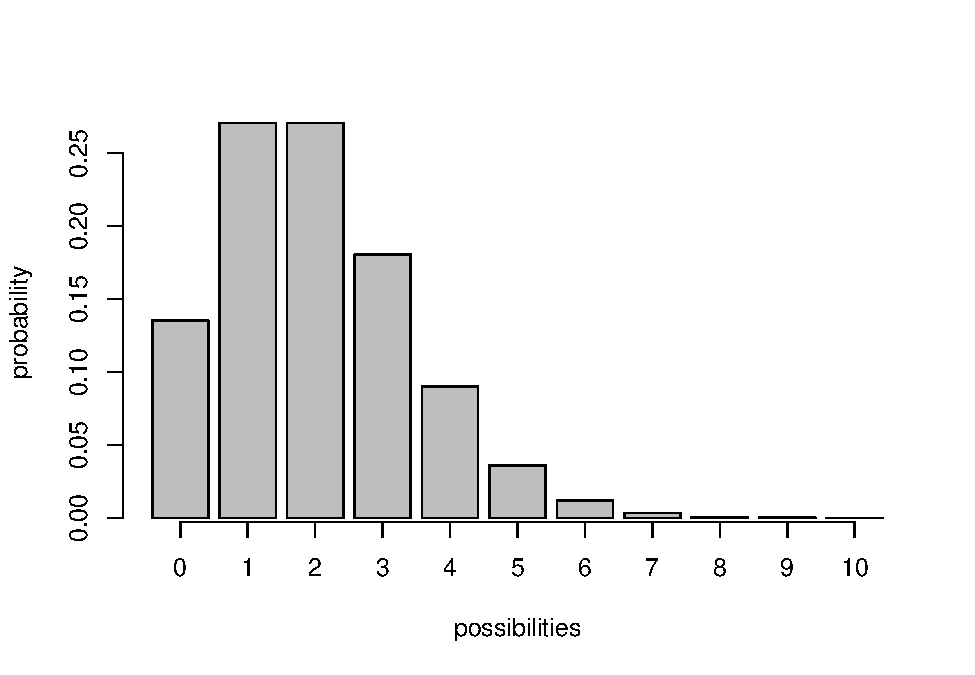
\includegraphics{LECTURE2_files/figure-latex/unnamed-chunk-17-1.pdf}

\hypertarget{cumulative-distribution-function}{%
\paragraph{Cumulative distribution
function}\label{cumulative-distribution-function}}

For continuous AND discrete probability distributions, \textbf{CDFs} -
Cumulative distribution functions (e.g.,
`pnorm',`pt',`pchisq',`pbinom',`ppois') give you the probability of
obtaining a value less than or equal to any particular value that could
be sampled under the distribution.

\begin{Shaded}
\begin{Highlighting}[]
\DocumentationTok{\#\# cumulative distribution function  }

    \CommentTok{\# for continuous distribution}
\FunctionTok{curve}\NormalTok{(}\FunctionTok{pt}\NormalTok{(x,}\AttributeTok{df=}\DecValTok{8}\NormalTok{),}\SpecialCharTok{{-}}\DecValTok{4}\NormalTok{,}\DecValTok{4}\NormalTok{,}\AttributeTok{xlab=}\StringTok{"possibilities"}\NormalTok{,}\AttributeTok{ylab=}\StringTok{\textquotesingle{}cumulative probability\textquotesingle{}}\NormalTok{)}
\end{Highlighting}
\end{Shaded}

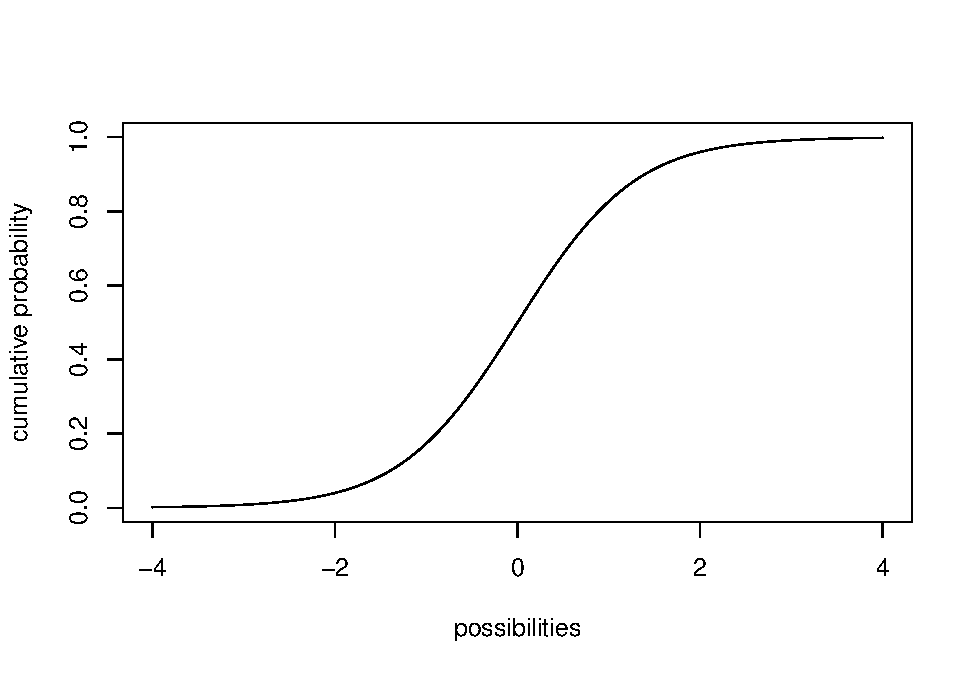
\includegraphics{LECTURE2_files/figure-latex/unnamed-chunk-18-1.pdf}

\begin{Shaded}
\begin{Highlighting}[]
    \CommentTok{\# for discrete distribution}
\NormalTok{x }\OtherTok{\textless{}{-}} \FunctionTok{barplot}\NormalTok{(}\FunctionTok{sapply}\NormalTok{(}\DecValTok{0}\SpecialCharTok{:}\DecValTok{10}\NormalTok{,}\ControlFlowTok{function}\NormalTok{(t) }\FunctionTok{ppois}\NormalTok{(t,}\DecValTok{2}\NormalTok{)),}\AttributeTok{xlab=}\StringTok{"possibilities"}\NormalTok{,}\AttributeTok{ylab=}\StringTok{\textquotesingle{}cumulative probability\textquotesingle{}}\NormalTok{)}
\FunctionTok{axis}\NormalTok{(}\DecValTok{1}\NormalTok{,}\AttributeTok{at=}\NormalTok{x,}\AttributeTok{labels=}\DecValTok{0}\SpecialCharTok{:}\DecValTok{10}\NormalTok{)}
\end{Highlighting}
\end{Shaded}

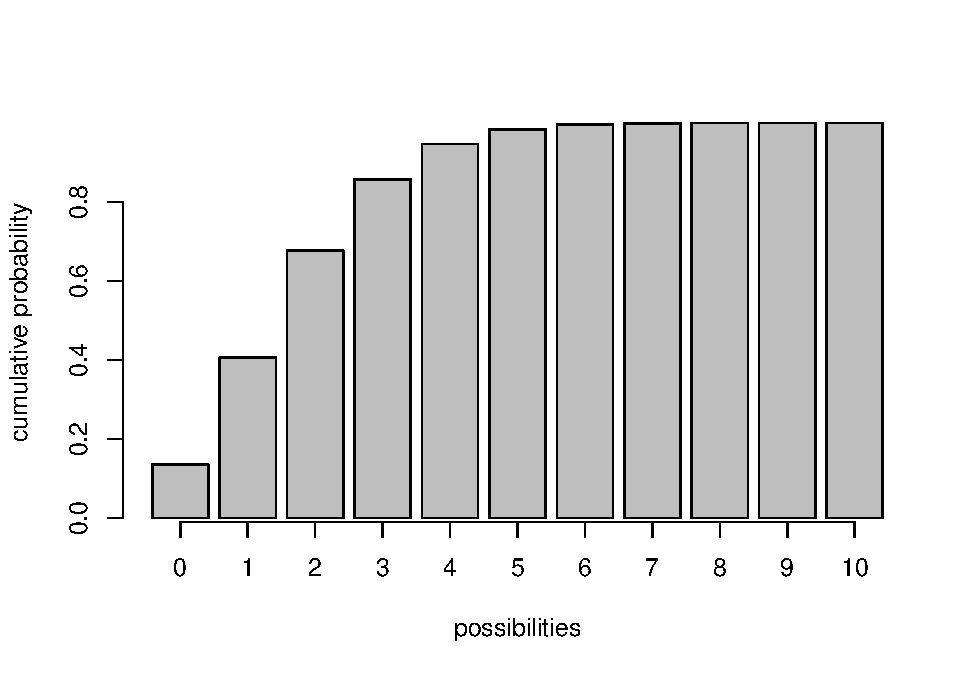
\includegraphics{LECTURE2_files/figure-latex/unnamed-chunk-18-2.pdf}

\hypertarget{quantile-functions}{%
\paragraph{Quantile functions}\label{quantile-functions}}

\textbf{Quantile functions} - inverse of CDF- give you the values below
which a specific percent of random samples should fall (e.g.,
`qnorm',`qt',`qpois',`qchisq'). The quantile function is the inverse of
the cumulative distribution function.

\begin{Shaded}
\begin{Highlighting}[]
\DocumentationTok{\#\# quantile function  }

    \CommentTok{\# for continuous distribution}
\FunctionTok{curve}\NormalTok{(}\FunctionTok{qt}\NormalTok{(x,}\AttributeTok{df=}\DecValTok{8}\NormalTok{),}\DecValTok{0}\NormalTok{,}\DecValTok{1}\NormalTok{,}\AttributeTok{xlab=}\StringTok{"cumulative probability"}\NormalTok{,}\AttributeTok{ylab=}\StringTok{\textquotesingle{}quantile\textquotesingle{}}\NormalTok{)}
\end{Highlighting}
\end{Shaded}

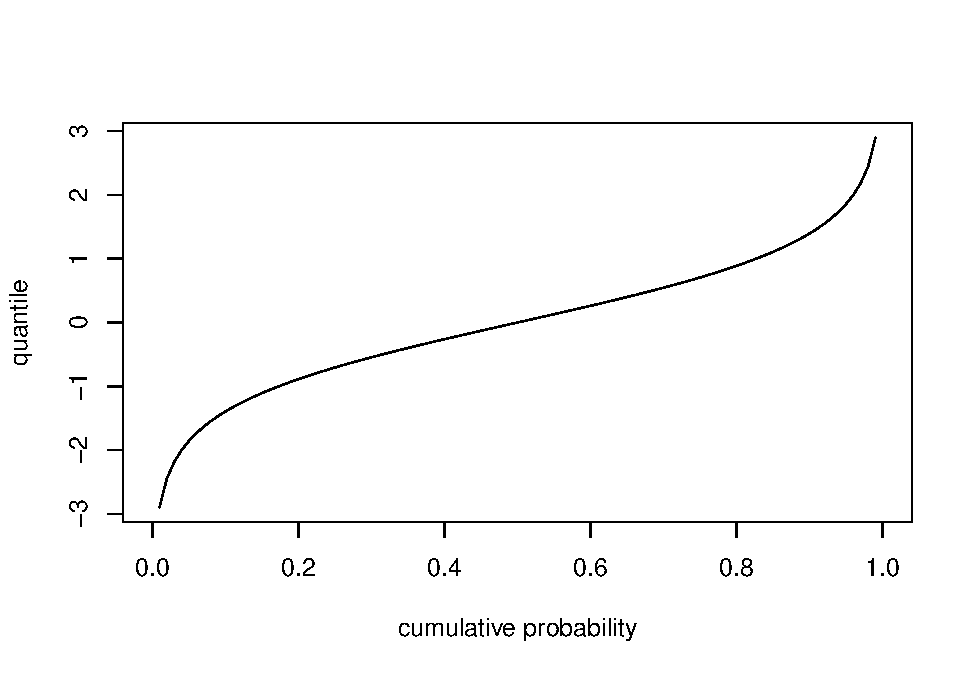
\includegraphics{LECTURE2_files/figure-latex/unnamed-chunk-19-1.pdf}

\begin{Shaded}
\begin{Highlighting}[]
    \CommentTok{\# for discrete distribution}
\FunctionTok{curve}\NormalTok{(}\FunctionTok{qpois}\NormalTok{(x,}\DecValTok{4}\NormalTok{),}\DecValTok{0}\NormalTok{,}\DecValTok{1}\NormalTok{,}\AttributeTok{xlab=}\StringTok{"cumulative probability"}\NormalTok{,}\AttributeTok{ylab=}\StringTok{\textquotesingle{}quantile\textquotesingle{}}\NormalTok{)}
\end{Highlighting}
\end{Shaded}

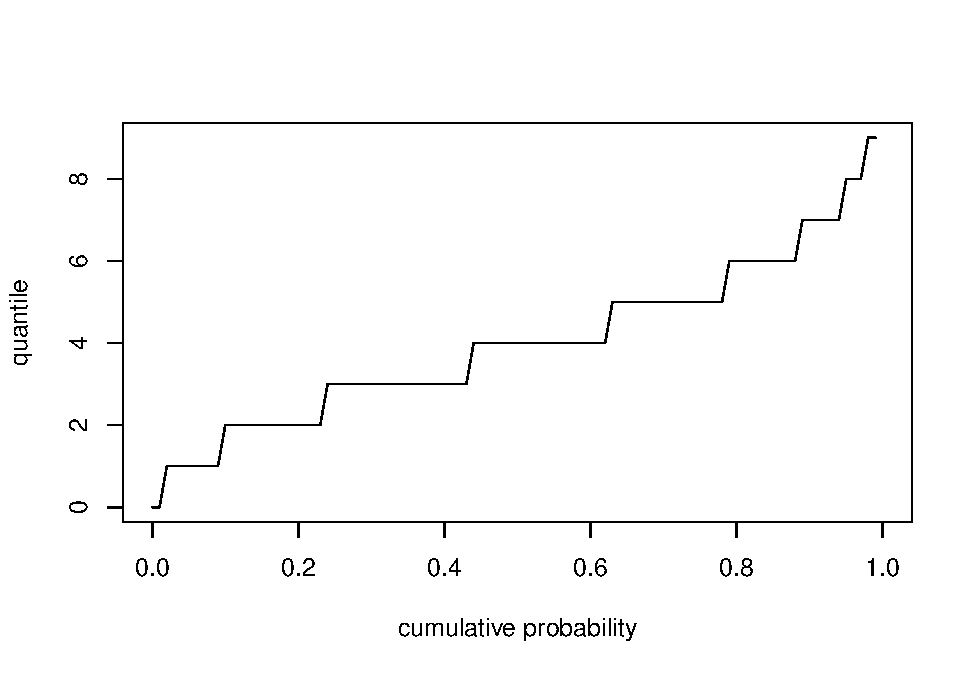
\includegraphics{LECTURE2_files/figure-latex/unnamed-chunk-19-2.pdf}

\hypertarget{moments}{%
\subsubsection{Moments}\label{moments}}

\textbf{Moments} are important descriptors of a distribution. The
collection of all the moments (of all orders, from 0 to infinity)
uniquely determines the shape of the distribution.

\begin{itemize}
\tightlist
\item
  The zeroth central moment
  (\(\int \left ( x-\mu \right )^{0}Prob(x)\partial x\)) is the total
  probability (i.e.~one),\\
\item
  The first central moment
  (\(\int \left ( x-\mu \right )^{1}Prob(x)\partial x\)) is
  \(\mu - \mu = 0\).\\
\item
  The second central moment
  (\(\int \left ( x-\mu \right )^{2}Prob(x)\partial x\)) is the
  variance.\\
\item
  The third central moment
  (\(\int \left ( \left (x-\mu \right )/\sigma \right )^{3}Prob(x)\partial x\))
  is the skewness.\\
\item
  The fourth central moment is the kurtosis.
\end{itemize}

\hypertarget{some-common-probability-distributions}{%
\subsubsection{Some common probability
distributions}\label{some-common-probability-distributions}}

Here are some common probability distributions. Pay particular attention
to the type of \emph{process} described by each distribution. The key to
using these distributions to represent random variables is to figure out
which statistical process best matches the ecological process you're
studying, then use that distribution. e.g., am I counting independent,
random events occurring in a fixed window of time or space (like
sampling barnacles in quadrats on an intertidal bench)? Then the
distribution of their occurrence is likely to follow a Poisson or
Negative Binomial distribution.

\hypertarget{binomial}{%
\paragraph{Binomial}\label{binomial}}

\begin{Shaded}
\begin{Highlighting}[]
\CommentTok{\# Binomial}

\NormalTok{size }\OtherTok{\textless{}{-}} \DecValTok{10}
\NormalTok{prob }\OtherTok{\textless{}{-}} \FloatTok{0.3}
\FunctionTok{rbinom}\NormalTok{(}\DecValTok{10}\NormalTok{,size,prob)}
\end{Highlighting}
\end{Shaded}

\begin{verbatim}
##  [1] 2 1 4 2 2 3 5 1 3 1
\end{verbatim}

\begin{Shaded}
\begin{Highlighting}[]
\NormalTok{xvals }\OtherTok{\textless{}{-}} \FunctionTok{seq}\NormalTok{(}\DecValTok{0}\NormalTok{,size,}\DecValTok{1}\NormalTok{)}
\NormalTok{probs }\OtherTok{\textless{}{-}} \FunctionTok{dbinom}\NormalTok{(xvals,size,prob)}
\FunctionTok{names}\NormalTok{(probs) }\OtherTok{\textless{}{-}}\NormalTok{ xvals}
               
\FunctionTok{barplot}\NormalTok{(probs,}\AttributeTok{ylab=}\StringTok{"Probability"}\NormalTok{,}\AttributeTok{main=}\StringTok{"Binomial distribution"}\NormalTok{)}
\end{Highlighting}
\end{Shaded}

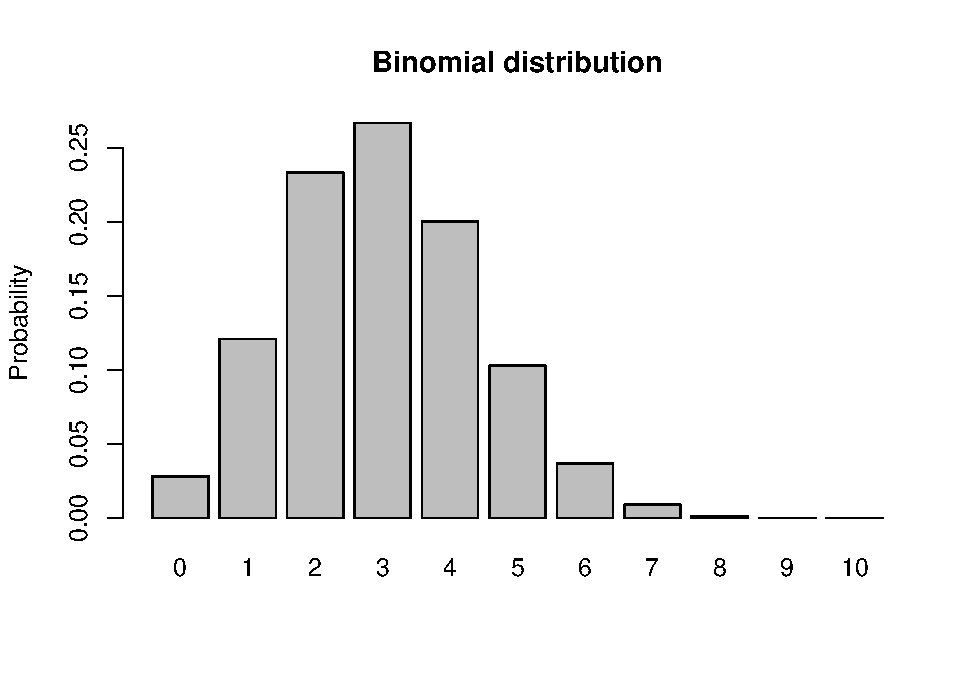
\includegraphics{LECTURE2_files/figure-latex/unnamed-chunk-20-1.pdf}

\begin{Shaded}
\begin{Highlighting}[]
\FunctionTok{barplot}\NormalTok{(}\FunctionTok{cumsum}\NormalTok{(probs),}\AttributeTok{ylab=}\StringTok{"Cumulative Probability"}\NormalTok{,}\AttributeTok{main=}\StringTok{"Binomial distribution"}\NormalTok{)   }\CommentTok{\# cumulative distribution}
\end{Highlighting}
\end{Shaded}

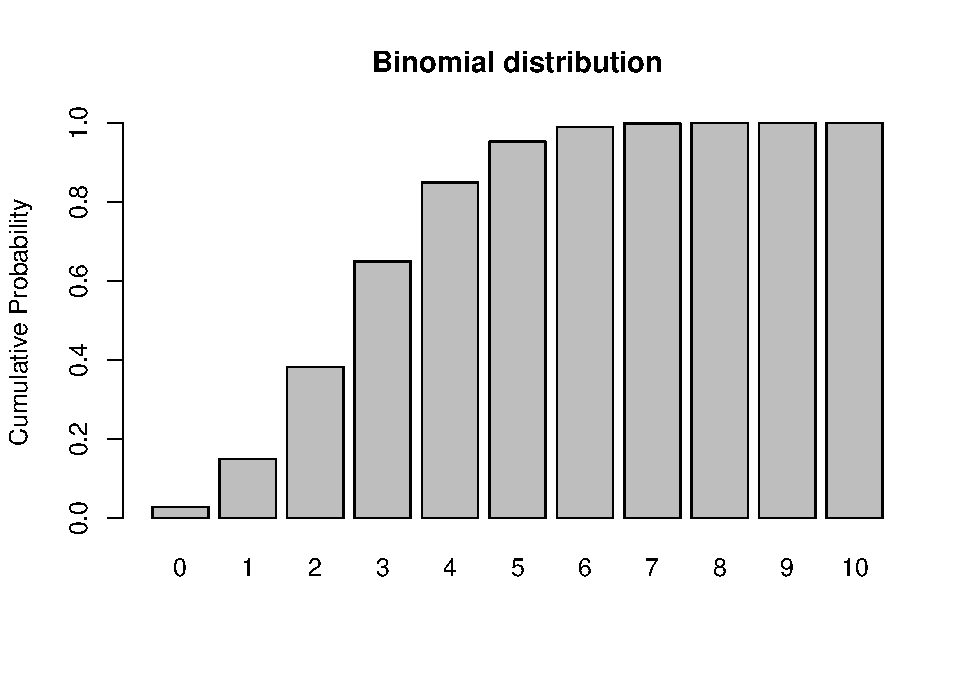
\includegraphics{LECTURE2_files/figure-latex/unnamed-chunk-20-2.pdf}

\begin{Shaded}
\begin{Highlighting}[]
\FunctionTok{sum}\NormalTok{(probs)   }\CommentTok{\# just to make sure it sums to 1!  Does it???}
\end{Highlighting}
\end{Shaded}

\begin{verbatim}
## [1] 1
\end{verbatim}

\hypertarget{normal}{%
\paragraph{Normal}\label{normal}}

\begin{Shaded}
\begin{Highlighting}[]
\CommentTok{\# Gaussian (normal)}

\NormalTok{mean }\OtherTok{=} \FloatTok{7.1}
\NormalTok{stdev }\OtherTok{=} \FloatTok{1.9}

\FunctionTok{rnorm}\NormalTok{(}\DecValTok{10}\NormalTok{,mean,stdev)}
\end{Highlighting}
\end{Shaded}

\begin{verbatim}
##  [1] 6.244913 6.800643 8.519310 5.887611 8.102712 6.944301 8.157094 7.323846 9.633420 7.703414
\end{verbatim}

\begin{Shaded}
\begin{Highlighting}[]
\FunctionTok{curve}\NormalTok{(}\FunctionTok{dnorm}\NormalTok{(x,mean,stdev),}\DecValTok{0}\NormalTok{,}\DecValTok{15}\NormalTok{)   }\CommentTok{\# probability density}
\end{Highlighting}
\end{Shaded}

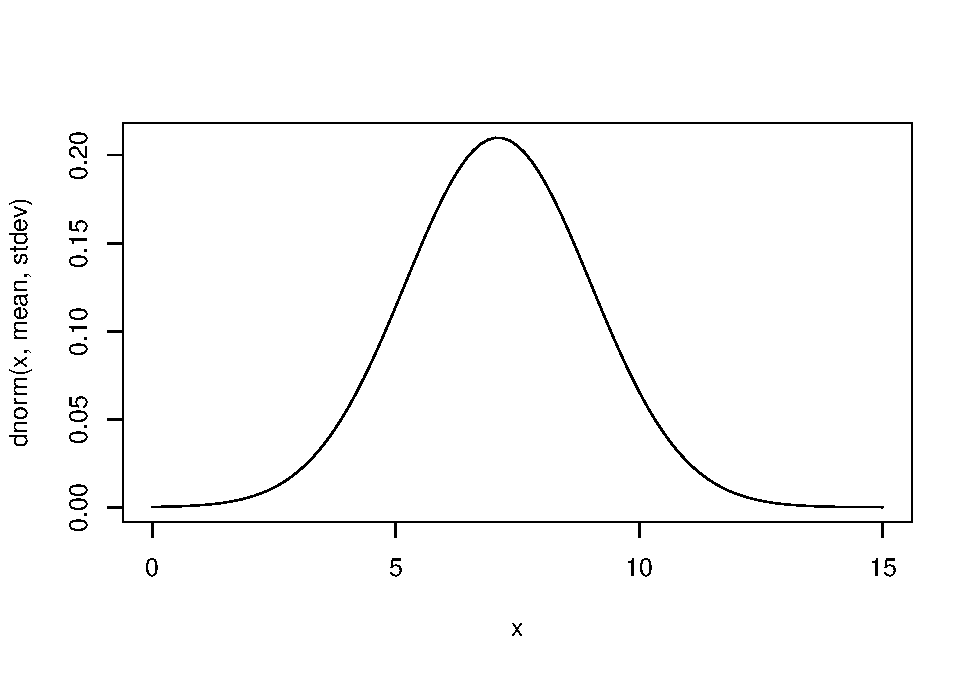
\includegraphics{LECTURE2_files/figure-latex/unnamed-chunk-21-1.pdf}

\begin{Shaded}
\begin{Highlighting}[]
\FunctionTok{curve}\NormalTok{(}\FunctionTok{pnorm}\NormalTok{(x,mean,stdev),}\DecValTok{0}\NormalTok{,}\DecValTok{15}\NormalTok{)   }\CommentTok{\# cumulative distribution}
\end{Highlighting}
\end{Shaded}

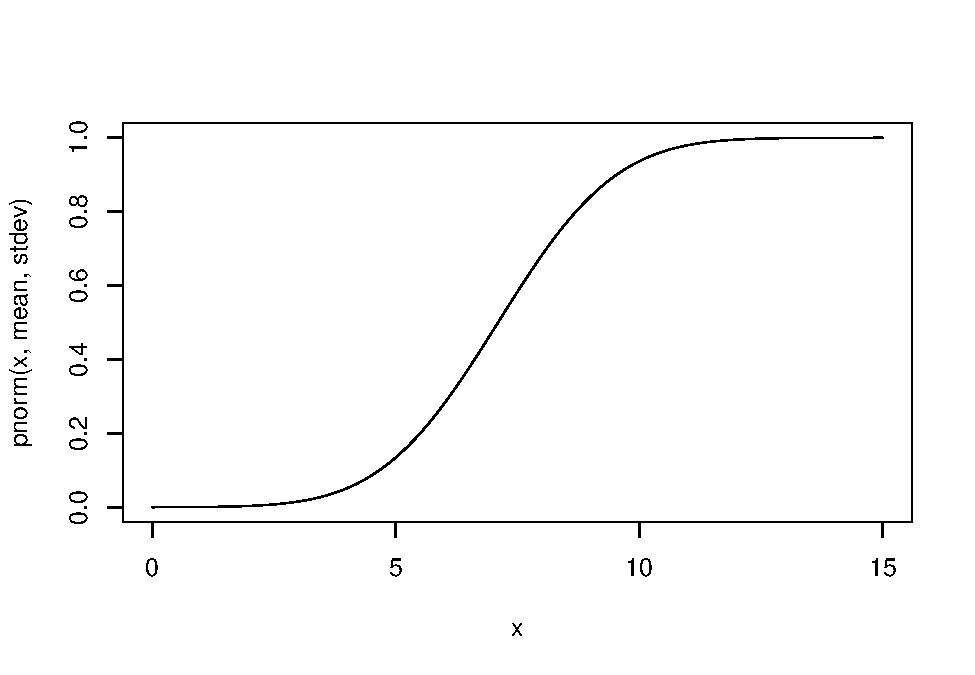
\includegraphics{LECTURE2_files/figure-latex/unnamed-chunk-21-2.pdf}

\begin{Shaded}
\begin{Highlighting}[]
\FunctionTok{integrate}\NormalTok{(}\AttributeTok{f=}\NormalTok{dnorm,}\AttributeTok{lower=}\SpecialCharTok{{-}}\ConstantTok{Inf}\NormalTok{,}\AttributeTok{upper=}\ConstantTok{Inf}\NormalTok{,}\AttributeTok{mean=}\NormalTok{mean,}\AttributeTok{sd=}\NormalTok{stdev)    }\CommentTok{\# just to make sure it integrates to 1!!}
\end{Highlighting}
\end{Shaded}

\begin{verbatim}
## 1 with absolute error < 1.1e-05
\end{verbatim}

\hypertarget{t-distribution}{%
\paragraph{t distribution}\label{t-distribution}}

\begin{Shaded}
\begin{Highlighting}[]
\CommentTok{\# t distribution}

\NormalTok{df }\OtherTok{=} \DecValTok{6}

\FunctionTok{rt}\NormalTok{(}\DecValTok{10}\NormalTok{,df)     }\CommentTok{\# random numbers from the t distribution}
\end{Highlighting}
\end{Shaded}

\begin{verbatim}
##  [1]  1.7730201 -0.4030480 -0.2326807  0.5326289  1.0121368 -0.8031428 -1.9359791  1.9138062  1.5393368
## [10] -2.1235209
\end{verbatim}

\begin{Shaded}
\begin{Highlighting}[]
\FunctionTok{curve}\NormalTok{(}\FunctionTok{dt}\NormalTok{(x,df),}\SpecialCharTok{{-}}\DecValTok{4}\NormalTok{,}\DecValTok{4}\NormalTok{)   }\CommentTok{\# probability density}
\end{Highlighting}
\end{Shaded}

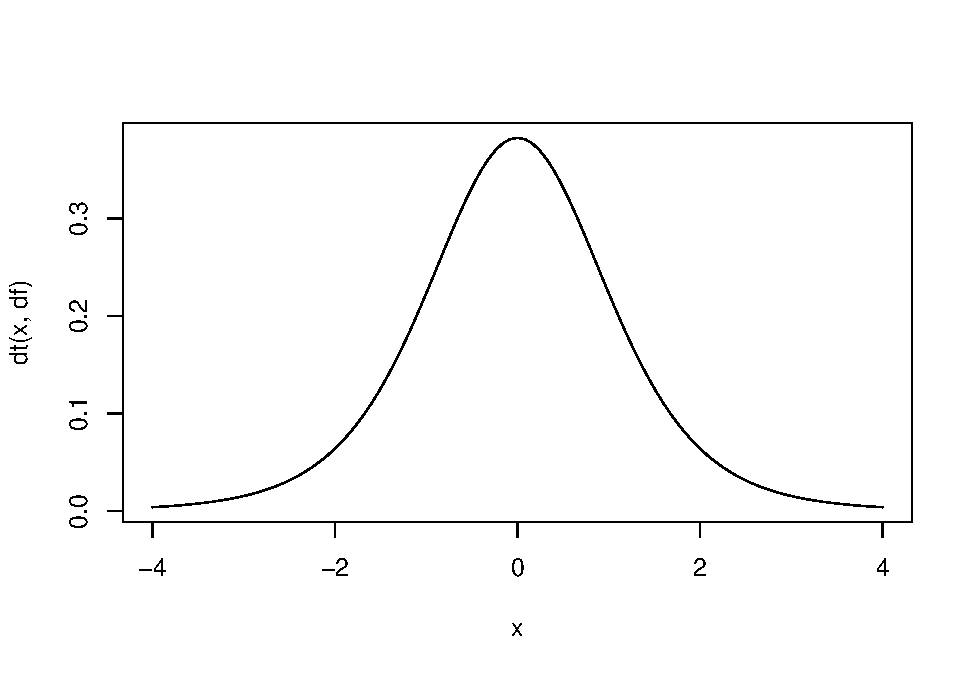
\includegraphics{LECTURE2_files/figure-latex/unnamed-chunk-22-1.pdf}

\begin{Shaded}
\begin{Highlighting}[]
\FunctionTok{curve}\NormalTok{(}\FunctionTok{pt}\NormalTok{(x,df),}\SpecialCharTok{{-}}\DecValTok{4}\NormalTok{,}\DecValTok{4}\NormalTok{)   }\CommentTok{\# cumulative distribution}
\end{Highlighting}
\end{Shaded}

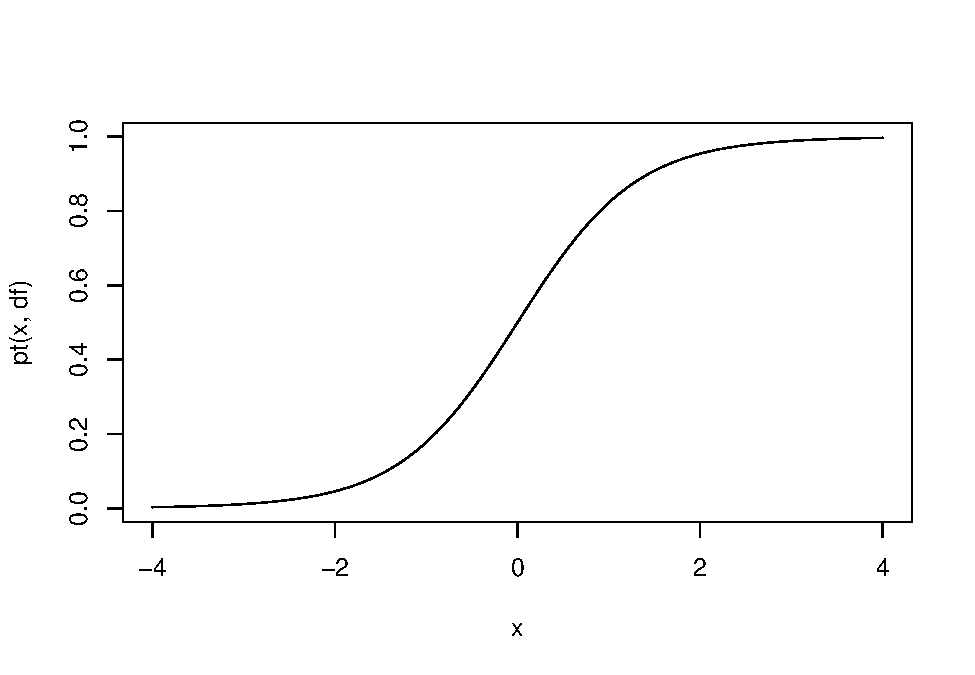
\includegraphics{LECTURE2_files/figure-latex/unnamed-chunk-22-2.pdf}

\begin{Shaded}
\begin{Highlighting}[]
\FunctionTok{integrate}\NormalTok{(}\AttributeTok{f=}\NormalTok{dt,}\AttributeTok{lower=}\SpecialCharTok{{-}}\ConstantTok{Inf}\NormalTok{,}\AttributeTok{upper=}\ConstantTok{Inf}\NormalTok{,}\AttributeTok{df=}\NormalTok{df)    }\CommentTok{\# just to make sure it integrates to 1!!}
\end{Highlighting}
\end{Shaded}

\begin{verbatim}
## 1 with absolute error < 1.9e-05
\end{verbatim}

\hypertarget{chi-squared-distribution}{%
\paragraph{Chi-squared distribution}\label{chi-squared-distribution}}

\begin{Shaded}
\begin{Highlighting}[]
\CommentTok{\# Chi{-}squared distribution}

\NormalTok{df }\OtherTok{=} \DecValTok{6}

\FunctionTok{rchisq}\NormalTok{(}\DecValTok{10}\NormalTok{,df)     }\CommentTok{\# random numbers from the chi squared distribution}
\end{Highlighting}
\end{Shaded}

\begin{verbatim}
##  [1]  0.8584865  3.4040866  5.1593658  4.7663263 11.9236727  4.2445110  3.2036503  4.3907526  4.4029836
## [10]  6.0182506
\end{verbatim}

\begin{Shaded}
\begin{Highlighting}[]
\FunctionTok{curve}\NormalTok{(}\FunctionTok{dchisq}\NormalTok{(x,df),}\DecValTok{0}\NormalTok{,}\DecValTok{15}\NormalTok{)   }\CommentTok{\# probability density}
\end{Highlighting}
\end{Shaded}

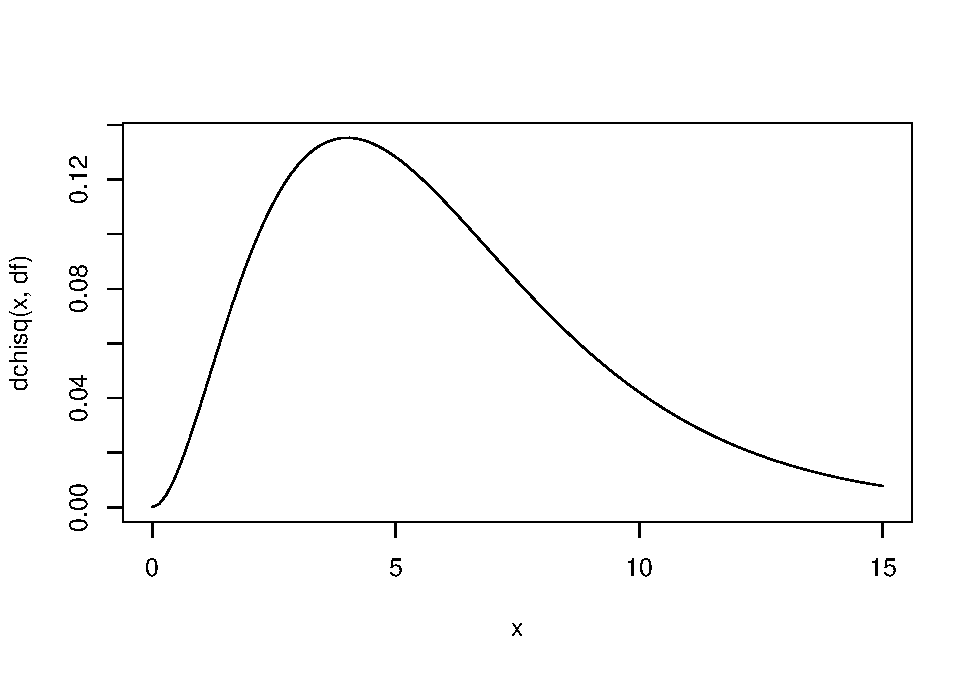
\includegraphics{LECTURE2_files/figure-latex/unnamed-chunk-23-1.pdf}

\begin{Shaded}
\begin{Highlighting}[]
\FunctionTok{curve}\NormalTok{(}\FunctionTok{pchisq}\NormalTok{(x,df),}\DecValTok{0}\NormalTok{,}\DecValTok{15}\NormalTok{)   }\CommentTok{\# cumulative distribution}
\end{Highlighting}
\end{Shaded}

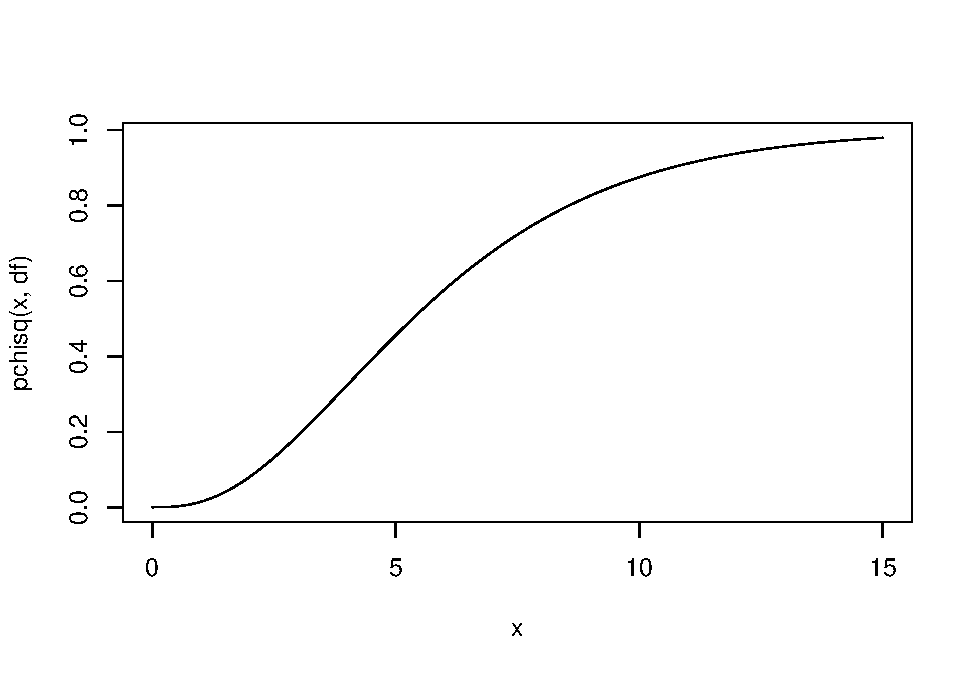
\includegraphics{LECTURE2_files/figure-latex/unnamed-chunk-23-2.pdf}

\begin{Shaded}
\begin{Highlighting}[]
\FunctionTok{integrate}\NormalTok{(}\AttributeTok{f=}\NormalTok{dchisq,}\AttributeTok{lower=}\DecValTok{0}\NormalTok{,}\AttributeTok{upper=}\ConstantTok{Inf}\NormalTok{,}\AttributeTok{df=}\NormalTok{df)    }\CommentTok{\# just to make sure it integrates to 1!!}
\end{Highlighting}
\end{Shaded}

\begin{verbatim}
## 1 with absolute error < 2.3e-05
\end{verbatim}

\hypertarget{exercise-in-class-not-graded}{%
\paragraph{Exercise (in class, not
graded):}\label{exercise-in-class-not-graded}}

Visualize (in R) the following distributions as above: Gamma,
Exponential, Lognormal, Negative Binomial.

\href{LECTURE3.html}{--go to next lecture--}

\end{document}
